\documentclass{vkr}
\usepackage[english, russian]{babel} % переносы
\usepackage{graphicx} % для вставки картинок
\graphicspath{{images/}} % путь к изображениям
\usepackage[hidelinks]{hyperref}
\usepackage{float} % определяет метод H для рисунка с переносом на следующую страницу, ели не помещается
\usepackage{pdflscape}
\addto{\captionsrussian}{\renewcommand{\refname}{СПИСОК ИСПОЛЬЗОВАННЫХ ИСТОЧНИКОВ}}
\usepackage{xltabular} % для вставки таблиц
\usepackage{makecell}
\renewcommand\theadfont{} % шрифт в /thead
\usepackage{array} % для определения новых типов столбцов таблиц
\newcolumntype{T}{>{\centering\arraybackslash}X} % новый тип столбца T - автоматическая ширина столбца с выравниванием по центру
\newcolumntype{R}{>{\raggedleft\arraybackslash}X} % новый тип столбца R - автоматическая ширина столбца с выравниванием по правому краю
\newcolumntype{C}[1]{>{\centering\let\newline\\\arraybackslash\hspace{0pt}}m{#1}} % новый тип столбца C - фиксированная ширина столбца с выравниванием по центру
\newcolumntype{r}[1]{>{\raggedleft\arraybackslash}p{#1}} % новый тип столбца r - фиксированная ширина столбца с выравниванием по правому краю
\newcommand{\centrow}{\centering\arraybackslash} % командой \centrow можно центрировать одну ячейку (заголовок) в столбце типа X или p, оставив в оcтальных ячейках другой тип выравнивания
\newcommand{\finishhead}{\endhead\hline\endlastfoot}
\newcommand{\continuecaption}[1]{\caption*{#1}\\ \hline }
\usepackage{etoolbox}
\AtBeginEnvironment{xltabular}{\refstepcounter{tablecnt}} % подсчет таблиц xltabular, обычные таблицы подсчитываются в классе

\usepackage[tableposition=top]{caption} % подпись таблицы вверху
\captionsetup{strut=off}
\setlength{\intextsep}{0pt} % Vertical space above & below [h] floats
\setlength{\textfloatsep}{0pt} % Vertical space below (above) [t] ([b]) floats
\DeclareCaptionLabelFormat{gostfigure}{Рисунок #2} %подпись рисунка
\DeclareCaptionLabelFormat{gosttable}{Таблица #2} %подпись таблицы
\DeclareCaptionLabelSeparator{gost}{~--~} %разделитель в рисунках и таблицах
\captionsetup{labelsep=gost}
\captionsetup[figure]{aboveskip=10pt,belowskip=4mm,justification=centering,labelformat=gostfigure} % настройка подписи рисунка
\captionsetup[table]{font={stretch=1.41},skip=0pt,belowskip=0pt,aboveskip=8.5pt,singlelinecheck=off,labelformat=gosttable} % настройка подписи таблицы

\setlength{\LTpre}{8mm} % отступ сверху таблицы
\setlength{\LTpost}{6mm} % отступ снизу таблицы

\usepackage{verbatim}


\usepackage{enumitem}
\setlist{nolistsep,wide=\parindent,itemindent=*} % отступы вокруг списков, выравнивание с учетом разделителя

\usepackage{color} %% это для отображения цвета в коде
\usepackage{listings} %% листинги кода
\setmonofont[Scale=0.7]{Verdana} % моноширный шрифт для листинга

\definecolor{codegreen}{rgb}{0,0.6,0}
\definecolor{codegray}{rgb}{0.5,0.5,0.5}
\definecolor{codepurple}{rgb}{0.58,0,0.82}

\lstset{ %
language=C,                 % выбор языка для подсветки (здесь это С)
numbers=left,               % где поставить нумерацию строк (слева\справа)
numberstyle=\tiny,           % размер шрифта для номеров строк
stepnumber=1,                   % размер шага между двумя номерами строк
numbersep=5pt,                % как далеко отстоят номера строк от подсвечиваемого кода
commentstyle=\color{codegreen},
keywordstyle=\color{magenta},
numberstyle=\tiny\color{codegray},
stringstyle=\color{codepurple},
basicstyle=\linespread{0.95}\ttfamily,
backgroundcolor=\color{white}, % цвет фона подсветки - используем \usepackage{color}
showspaces=false,            % показывать или нет пробелы специальными отступами
showstringspaces=false,      % показывать или нет пробелы в строках
showtabs=false,             % показывать или нет табуляцию в строках
frame=single,              % рисовать рамку вокруг кода
tabsize=2,                 % размер табуляции по умолчанию равен 2 пробелам
captionpos=t,              % позиция заголовка вверху [t] или внизу [b] 
breaklines=true,           % автоматически переносить строки (да\нет)
breakatwhitespace=false, % переносить строки только если есть пробел
escapeinside={\%*}{*)}   % если нужно добавить комментарии в коде
}

\makeatletter % чтобы допускались русские комментарии в листингах
\lst@InputCatcodes
\def\lst@DefEC{%
 \lst@CCECUse \lst@ProcessLetter
  ^^80^^81^^82^^83^^84^^85^^86^^87^^88^^89^^8a^^8b^^8c^^8d^^8e^^8f%
  ^^90^^91^^92^^93^^94^^95^^96^^97^^98^^99^^9a^^9b^^9c^^9d^^9e^^9f%
  ^^a0^^a1^^a2^^a3^^a4^^a5^^a6^^a7^^a8^^a9^^aa^^ab^^ac^^ad^^ae^^af%
  ^^b0^^b1^^b2^^b3^^b4^^b5^^b6^^b7^^b8^^b9^^ba^^bb^^bc^^bd^^be^^bf%
  ^^c0^^c1^^c2^^c3^^c4^^c5^^c6^^c7^^c8^^c9^^ca^^cb^^cc^^cd^^ce^^cf%
  ^^d0^^d1^^d2^^d3^^d4^^d5^^d6^^d7^^d8^^d9^^da^^db^^dc^^dd^^de^^df%
  ^^e0^^e1^^e2^^e3^^e4^^e5^^e6^^e7^^e8^^e9^^ea^^eb^^ec^^ed^^ee^^ef%
  ^^f0^^f1^^f2^^f3^^f4^^f5^^f6^^f7^^f8^^f9^^fa^^fb^^fc^^fd^^fe^^ff%
  ^^^^20ac^^^^0153^^^^0152%
  % Basic Cyrillic alphabet coverage
  ^^^^0410^^^^0411^^^^0412^^^^0413^^^^0414^^^^0415^^^^0416^^^^0417%
  ^^^^0418^^^^0419^^^^041a^^^^041b^^^^041c^^^^041d^^^^041e^^^^041f%
  ^^^^0420^^^^0421^^^^0422^^^^0423^^^^0424^^^^0425^^^^0426^^^^0427%
  ^^^^0428^^^^0429^^^^042a^^^^042b^^^^042c^^^^042d^^^^042e^^^^042f%
  ^^^^0430^^^^0431^^^^0432^^^^0433^^^^0434^^^^0435^^^^0436^^^^0437%
  ^^^^0438^^^^0439^^^^043a^^^^043b^^^^043c^^^^043d^^^^043e^^^^043f%
  ^^^^0440^^^^0441^^^^0442^^^^0443^^^^0444^^^^0445^^^^0446^^^^0447%
  ^^^^0448^^^^0449^^^^044a^^^^044b^^^^044c^^^^044d^^^^044e^^^^044f%
  ^^^^0401^^^^0451%
  %%%
  ^^00}
\lst@RestoreCatcodes
\makeatother


% Режим шаблона (должен быть включен один из трех)
\ВКРtrue
%\Практикаtrue
%\Курсоваяtrue

\newcommand{\Дисциплина}{<<Проектирование и архитектура программных систем>>} % для курсовой
\newcommand{\КодСпециальности}{09.03.04} % Курсовая
\newcommand{\Специальность}{Программная инженерия} % Курсовая
\newcommand{\Тема}{Программно-информационная система для управления энергопотреблением} % ВКР Курсовая
\newcommand{\ТемаВтораяСтрока}{в зданиях}
\newcommand{\ГдеПроводитсяПрактика}{Юго-Западном государственном университете} % для практики
\newcommand{\РуководительПрактПредпр}{Куркина А. В.} % для практики
\newcommand{\ДолжнРуководительПрактПредпр}{директор} % для практики
\newcommand{\РуководительПрактУнивер}{Чаплыгин А. А.} % для практики
\newcommand{\ДолжнРуководительПрактУнивер}{к.т.н. доцент} % для практики
\newcommand{\Автор}{М. С. Черенков}
\newcommand{\АвторРод}{Черенкова М.С.}
\newcommand{\АвторПолностьюРод}{Черенкова Михаила Сергеевича} % для практики
\newcommand{\Шифр}{19-06-0462}
\newcommand{\Курс}{5} % для практики
\newcommand{\Группа}{ПО-92з}
\newcommand{\Руководитель}{И. Н. Ефремова} % для ВКР и курсовой
\newcommand{\Нормоконтроль}{А. А. Чаплыгин} % для ВКР
\newcommand{\ЗавКаф}{А. В. Малышев} % для ВКР
\newcommand{\ДатаПриказа}{«13» ноября 2023~г.} % для ВКР
\newcommand{\НомерПриказа}{5166-с} % для ВКР
\newcommand{\СрокПредоставления}{«21» декабря 2023~г.} % для ВКР, курсового

\begin{document}
\maketitle
\ifПрактика{}\else{
   \newpage
\begin{center}
\large\textbf{Минобрнауки России}

\large\textbf{Юго-Западный государственный университет}
\vskip 1em
\normalsize{Кафедра программной инженерии}
\vskip 1em
\ifВКР{
        \begin{flushright}
        \begin{tabular}{p{.4\textwidth}}
        \centrow УТВЕРЖДАЮ: \\
        \centrow Заведующий кафедрой \\
        \hrulefill \\
        \setarstrut{\footnotesize}
        \centrow\footnotesize{(подпись, инициалы, фамилия)}\\
        \restorearstrut
        «\underline{\hspace{1cm}}»
        \underline{\hspace{3cm}}
        20\underline{\hspace{1cm}} г.\\
        \end{tabular}
        \end{flushright}
        }\fi
\end{center}
\vspace{1em}
  \begin{center}
  \large
\ifВКР{
ЗАДАНИЕ НА ВЫПУСКНУЮ КВАЛИФИКАЦИОННУЮ РАБОТУ
  ПО ПРОГРАММЕ БАКАЛАВРИАТА}
  \else
ЗАДАНИЕ НА КУРСОВУЮ РАБОТУ (ПРОЕКТ)
\fi
\normalsize
  \end{center}
\vspace{1em}
{\parindent0pt
  Студента \АвторРод, шифр\ \Шифр, группа \Группа
  
1. Тема «\Тема\ \ТемаВтораяСтрока»
\ifВКР{
утверждена приказом ректора ЮЗГУ от \ДатаПриказа\ № \НомерПриказа
}\fi.

2. Срок предоставления работы к защите \СрокПредоставления

3. Исходные данные для создания программной системы:

3.1. Перечень решаемых задач:}

\renewcommand\labelenumi{\theenumi)}

\begin{enumerate}
 
\item Проанализировать энергетическую инфраструктуру здания.
\item Провести анализ энергоснабжения здания, включая источники энергии, сетевые связи и оборудование.
\item Исследовать энергопотребление в различных зонах здания (освещение, отопление, кондиционирование и т.д.).
		
\item Разработать концептуальную модель программно-информационной системы управления энергопотреблением на основе современных подходов к энергетическому менеджменту.
\item Учесть возможности сбора данных о энергопотреблении с использованием сенсоров и умных устройств.
\item Разработать модель управления, основанную на данных о пиковых нагрузках, энергосбережении и оптимизации расходов.

\item Спроектировать программную систему управления энергопотреблением в зданиях.
\item Определить требования к программному обеспечению для мониторинга и управления энергосистемой здания.
\item Разработать архитектуру системы, включая взаимодействие с умными устройствами, базой данных и пользовательским интерфейсом.

\item Сконструировать и протестировать программную систему управления энергопотреблением в зданиях.
\item Разработать прототип программы для сбора, анализа и визуализации данных об энергопотреблении.
\item Провести тестирование системы на эффективность мониторинга, управления и оптимизации энергопотребления.

\end{enumerate}

{\parindent0pt
  3.2. Входные данные и требуемые результаты для программы:}

\begin{enumerate}

\item Входными данными для программной системы являются: данные о потреблении энергии различными зонами здания; технические характеристики энергетического оборудования; информация об энергетических стандартах и требованиях; данные о тарифах на энергоресурсы; информация о текущих ресурсах и запасах энергии.

\item Выходными данными для программной системы являются: оптимизированный график энергопотребления; отчеты по эффективности использования энергии; предупреждения и уведомления о возможных сбоях или неэффективном использовании энергии; визуализация данных по энергопотреблению для принятия управленческих решений.

\end{enumerate}

{\parindent0pt

  4. Содержание работы (по разделам):
  
  4.1. Введение
  
  4.1. Анализ предметной области
  
4.2. Техническое задание: основание для разработки, назначение разработки,
требования к программной системе, требования к оформлению документации.

4.3. Технический проект: общие сведения о программной системе, проект
данных программной системы, проектирование архитектуры программной системы, проектирование пользовательского интерфейса программной системы.

4.4. Рабочий проект: спецификация компонентов и классов программной системы, тестирование программной системы, сборка компонентов программной системы.

4.5. Заключение

4.6. Список использованных источников

5. Перечень графического материала:

\списокПлакатов

\vskip 2em
\begin{tabular}{p{6.8cm}C{3.8cm}C{4.8cm}}
Руководитель \ifВКР{ВКР}\else работы (проекта) \fi & \lhrulefill{\fill} & \fillcenter\Руководитель\\
\setarstrut{\footnotesize}
& \footnotesize{(подпись, дата)} & \footnotesize{(инициалы, фамилия)}\\
\restorearstrut
Задание принял к исполнению & \lhrulefill{\fill} & \fillcenter\Автор\\
\setarstrut{\footnotesize}
& \footnotesize{(подпись, дата)} & \footnotesize{(инициалы, фамилия)}\\
\restorearstrut
\end{tabular}
}

\renewcommand\labelenumi{\theenumi.}

   \abstract{РЕФЕРАТ}

Объем работы равен \formbytotal{lastpage}{страниц}{е}{ам}{ам}. Работа содержит \formbytotal{figurecnt}{иллюстраци}{ю}{и}{й}, \formbytotal{tablecnt}{таблиц}{у}{ы}{}, \arabic{bibcount} библиографических источников и \formbytotal{числоПлакатов}{лист}{}{а}{ов} графического материала. Количество приложений – 2. Графический материал представлен в приложении А. Фрагменты исходного кода представлены в приложении Б.

Перечень ключевых слов: энергопотребление, управление энергоресурсами, программно-информационная система, энергетическая инфраструктура, умные устройства, оптимизация энергопотребления, мониторинг, энергетический менеджмент.

Объектом разработки является программно-информационная система для управления энергопотреблением в зданиях.

Целью выпускной квалификационной работы является создание эффективной системы, позволяющей контролировать и оптимизировать энергопотребление в зданиях, с учетом различных зон и источников энергии.

В ходе разработки системы были выполнены следующие этапы:
\begin{enumerate}
	\item Анализ энергетической инфраструктуры здания, включая источники энергии и оборудование.
	\item Разработка концептуальной модели системы управления энергопотреблением, учитывающей современные подходы к энергетическому менеджменту.
	\item Спроектирована программная система, включая архитектуру, взаимодействие с умными устройствами и пользовательским интерфейсом.
	\item Сконструирована и протестирована программа для мониторинга, управления и оптимизации энергопотребления.
\end{enumerate}

Входными данными для системы являются информация о потреблении энергии различными зонами здания, технические характеристики оборудования, данные о тарифах и стандартах. Выходные данные включают оптимизированный график энергопотребления, отчеты и предупреждения.

Разработанная программно-информационная система предоставляет эффективные инструменты для управления энергопотреблением в зданиях, способствуя оптимизации расходов и повышению энергетической эффективности.

\selectlanguage{english}
\abstract{ABSTRACT}
  
The volume of work is \formbytotal{lastpage}{page}{}{s}{s}. The work contains \formbytotal{figurecnt}{illustration}{}{s}{s}, \formbytotal{tablecnt}{table}{}{s}{s}, \arabic{bibcount} bibliographic sources and \formbytotal{числоПлакатов}{sheet}{}{s}{s} of graphic material. The number of applications is 2. The graphic material is presented in annex A. The layout of the site, including the connection of components, is presented in annex B.

List of keywords: energy consumption, energy resource management, software information system, energy infrastructure, smart devices, energy consumption optimization, monitoring, energy management.

The object of development is a software information system designed for managing energy consumption in buildings.

The objective of the work is to create an effective system capable of monitoring and optimizing energy consumption in buildings, considering various zones and energy sources.

The development stages of the system included:
\begin{enumerate}
	\item Analysis of the energy infrastructure of the building, encompassing energy sources and equipment.
	\item Development of a conceptual model for energy consumption management system, taking into account modern approaches to energy management.
	\item Design of the software system, including architecture, interaction with smart devices, and user interface.
	\item Construction and testing of the program for monitoring, management, and optimization of energy consumption.
\end{enumerate}

Input data for the system include information on energy consumption in different building zones, technical characteristics of equipment, data on tariffs, and standards. Output data consist of an optimized energy consumption schedule, reports, and warnings.

The developed software information system provides efficient tools for managing energy consumption in buildings, contributing to cost optimization and increased energy efficiency.
\selectlanguage{russian}
}\fi
\tableofcontents
\section*{ОБОЗНАЧЕНИЯ И СОКРАЩЕНИЯ}

ПИС -- программно-информационная система.

ЭИ -- энергетическая инфраструктура.

УУ -- умные устройства.

ОЭ -- оптимизация энергопотребления.

МЭ -- мониторинг энергопотребления.

ГЭ -- график энергопотребления.

РА -- расходы энергии.

ВЭ -- визуализация энергопотребления.

ТД -- технические данные.

СУЭ -- система управления энергопотреблением.

ПЭ -- потребление энергии.
\ifПрактика{}\else{\section*{ВВЕДЕНИЕ}
\addcontentsline{toc}{section}{ВВЕДЕНИЕ}

В современном мире, где энергетические ресурсы становятся все более дефицитными и ценными, эффективное управление энергопотреблением в зданиях приобретает особенное значение. Для достижения устойчивости и снижения негативного воздействия на окружающую среду необходимы инновационные подходы, способные совмещать современные технологии и информационные системы. В этом контексте вступает в игру Программно-информационная система для управления энергопотреблением в зданиях, представляя собой передовое решение, направленное на оптимизацию энергетической эффективности и уменьшение воздействия на климат.

Эта интегрированная система предназначена для комплексного мониторинга, анализа и управления энергопотреблением в зданиях различного назначения, включая офисные здания, торговые центры, промышленные объекты и жилые комплексы. С ее помощью пользователи получают возможность в режиме реального времени отслеживать энергетические показатели, выявлять неэффективные потребители, оптимизировать расход электроэнергии и, таким образом, значительно снижать эксплуатационные расходы.

Основные преимущества программы включают в себя интеллектуальное управление системами освещения, отопления, вентиляции и кондиционирования воздуха, а также возможность удаленного доступа и управления через веб-интерфейс. Это позволяет адаптировать энергопотребление под конкретные потребности, минимизировать потери энергии и создавать оптимальные условия для жизни и работы.

Программно-информационная система для управления энергопотреблением в зданиях не только способствует рациональному использованию ресурсов, но также является важным шагом в направлении создания устойчивого и энергоэффективного общества. Современные технологии в области управления энергопотреблением становятся неотъемлемой частью стратегии устойчивого развития, и наша программа является ключевым инструментом в этом процессе.

Кроме того, Программно-информационная система (ПИС) для управления энергопотреблением в зданиях обеспечивает функционал сбора и анализа данных, что позволяет выявлять тенденции в потреблении энергии и предоставляет ценную информацию для принятия стратегических решений. Алгоритмы помощника встроенного в систему позволяют автоматически оптимизировать процессы управления, учитывая изменяющиеся потребности и внешние факторы.

Безопасность данных является ключевым аспектом работы системы. Программа предусматривает современные методы шифрования и механизмы защиты конфиденциальности, обеспечивая полную безопасность информации о потреблении энергии и других важных параметрах здания.

\emph{Цель данной работы} заключается в создании эффективной программно-информационной системы, способной мониторинга, управления и оптимизации энергопотребления в различных зонах зданий. Для достижения этой цели необходимо решить ряд\emph{ ключевых задач:}
\begin{itemize}
	\item Провести анализ энергетической инфраструктуры зданий с учетом различных источников энергии и зон потребления.
	\item Разработать концептуальную модель программной системы управления энергопотреблением, основанную на передовых методах энергетического менеджмента.
	\item Спроектировать программную систему, включая архитектуру, взаимодействие с умными устройствами и пользовательский интерфейс.
	\item Сконструировать и протестировать программную систему, обеспечивающую эффективное управление и мониторинг энергопотребления.
\end{itemize}

\emph{Структура и объем работы.} Отчет состоит из введения, 4 разделов основной части, заключения, списка использованных источников, 2 приложений. Текст выпускной квалификационной работы равен \formbytotal{page}{страниц}{е}{ам}{ам}.

\emph{Во введении} сформулирована цель работы, поставлены задачи разработки, описана структура работы, приведено краткое содержание каждого из разделов.

\emph{В первом разделе} на стадии описания технической характеристики предметной области приводится сбор информации о деятельности компании, для которой осуществляется разработка сайта.

\emph{Во втором разделе} на стадии технического задания приводятся требования к разрабатываемому сайту.

\emph{В третьем разделе} на стадии технического проектирования представлены проектные решения для web-сайта.

\emph{В четвертом разделе} приводится список классов и их методов, использованных при разработке сайта, производится тестирование разработанного сайта.

В заключении излагаются основные результаты работы, полученные в ходе разработки.

В приложении А представлен графический материал.
В приложении Б представлены фрагменты исходного кода. 
}\fi
\section{Анализ предметной области}
\subsection{Тенденции в энергопотреблении зданий}

Энергопотребление в современных зданиях охватывает широкий спектр аспектов, начиная от примитивных электрических устройств и заканчивая сложными системами умного дома. С ростом населения и городской застройки увеличивается спрос на энергию, что ставит перед нами задачу разработки эффективных и устойчивых решений для управления этим потреблением.

Системы отопления, вентиляции и кондиционирования в современных зданиях стали неотъемлемой частью обеспечения комфортных условий проживания и работы. Однако, их энергозатраты могут быть значительными, особенно при неэффективном использовании или устаревших технологиях. Разработка более энергоэффективных систем и внедрение интеллектуальных алгоритмов управления помогут снизить негативное воздействие на окружающую среду.

В свете современных тенденций также становится важным внедрение возобновляемых источников энергии в зданиях. Солнечные панели, ветрогенераторы и другие альтернативные источники играют ключевую роль в создании устойчивых, экологически чистых систем энергоснабжения. Их внедрение требует не только технической экспертизы, но и поддержки со стороны законодательства и общественного сознания.

Кроме того, с увеличением количества "умных" устройств в зданиях, сбор и анализ данных о потреблении энергии становятся важным инструментом для оптимизации эффективности. Использование сенсоров, интернета вещей и технологий искусственного интеллекта позволяет создавать адаптивные системы, способные предсказывать и реагировать на изменения в потреблении энергии, что в итоге снижает издержки и негативное воздействие на окружающую среду.

\subsection{Источники энергии и их влияние}

Разнообразие источников энергии, которые применяются в современных зданиях, включает в себя электроэнергию, тепловую энергию, а также возобновляемые источники. Эта разнообразная палитра выбора создает сложную динамику в энергетической инфраструктуре зданий, требуя тщательного анализа влияния каждого источника на общую эффективность системы энергоснабжения.

Электроэнергия, как один из основных источников, обеспечивает функционирование разнообразных устройств и систем внутри здания. Однако, зависимость от традиционных источников электроэнергии, таких как ископаемые топлива, может привести к негативным экологическим последствиям. В связи с этим, переход к более чистым источникам, таким как солнечная и ветровая энергия, становится важным шагом в снижении углеродного следа зданий.

Тепловая энергия, используемая для обеспечения отопления и горячего водоснабжения, также подвергается пересмотру в контексте устойчивости. Внедрение технологий, основанных на использовании геотермальной энергии или других возобновляемых источников, может не только снизить нагрузку на традиционные системы, но и сделать здания более экологически дружелюбными.

Возобновляемые источники энергии, такие как солнечная и ветровая энергия, играют ключевую роль в создании устойчивых систем энергоснабжения. Их использование содействует не только сокращению выбросов углерода, но и обеспечению независимости от изменений цен на традиционные источники энергии.

\subsection{Зоны потребления и мониторинг энергопотребления}

Внутри современных зданий существует многообразие зон, каждая из которых обладает уникальными потребностями в энергии. Эти зоны могут варьироваться от офисных пространств до жилых кварталов, а каждая из них требует индивидуального и оптимизированного подхода к энергоснабжению. Мониторинг энергопотребления в каждой из этих зон становится ключевым инструментом для выявления уникальных особенностей и определения возможностей для оптимизации энергетических процессов.

Офисные пространства, например, могут подвергаться резким изменениям в потреблении энергии в зависимости от времени суток и дня недели. Мониторинг, анализирующий эти изменения, позволяет предпринимать целенаправленные меры по снижению энергопотребления в периоды низкой активности, таким образом, повышая общую эффективность здания.

В жилых квартирах и домах, особенности потребления энергии могут зависеть от привычек и активности жителей. Точное измерение и анализ энергопотребления в этих зонах позволяют предоставлять персонализированные рекомендации по энергосбережению для жильцов, создавая комфортные условия без излишних затрат.

Мониторинг также обеспечивает возможность выявления неэффективных систем и устройств, способствуя своевременной замене или модернизации. Предоставление детальной информации о зонах потребления дает возможность инженерам и администраторам зданий точно настраивать системы управления энергопотреблением в соответствии с потребностями каждой конкретной зоны.

\subsection{Умные устройства и технологии}

Внедрение умных устройств и передовых технологий в здания – неотъемлемая часть современных энергосберегающих и устойчивых практик. Системы умного освещения, автоматизированные системы отопления и кондиционирования создают интеллектуальное окружение, которое может не только повысить комфорт, но и существенно снизить энергопотребление.

Системы умного освещения являются примером эффективного использования технологий для оптимизации энергии. Датчики движения и системы автоматического выключения не только обеспечивают освещение только в тех зонах, где оно действительно нужно, но и могут адаптироваться к внешним условиям, таким как естественное освещение из окон. Это позволяет снизить излишнее освещение и улучшить общую энергоэффективность.

Автоматизированные системы отопления и кондиционирования также играют важную роль в оптимизации энергопотребления зданий. Использование сенсоров для мониторинга температуры, влажности и других параметров позволяет точно регулировать условия в каждой зоне, реагируя на потребности и предотвращая избыточное потребление энергии.

Современные умные технологии также включают в себя системы управления энергопотреблением с использованием искусственного интеллекта. Эти системы могут анализировать данные о потреблении энергии в реальном времени, прогнозировать требования и автоматически оптимизировать работу устройств для достижения максимальной эффективности.

\subsection{Вызовы и требования к системе управления энергопотреблением}

Анализ предметной области энергопотребления в зданиях выдвигает перед нами ряд значительных вызовов, которые требуют системного подхода для достижения энергетической эффективности, устойчивости и соблюдения экологических стандартов. В этом контексте, требования к системе управления энергопотреблением становятся ключевым инструментом для успешного справления с вызовами современной энергетики.

Необходимость снижения затрат на энергию выступает в роли актуальной задачи, особенно в условиях растущего спроса на энергию и ограниченных ресурсов. Системы управления должны обеспечивать точный мониторинг и анализ энергопотребления в режиме реального времени, а также предоставлять механизмы для выявления и устранения избыточного потребления.

Увеличение устойчивости энергоснабжения требует решений, способных эффективно взаимодействовать с возобновляемыми источниками энергии, а также предоставлять надежную и устойчивую поддержку в случае возможных сбоев в сети. Гибкость и адаптивность становятся ключевыми элементами для эффективной интеграции разнообразных источников энергии и обеспечения устойчивости энергоснабжения.

Соблюдение экологических стандартов выходит на передний план, учитывая растущую осведомленность о климатических изменениях и необходимость снижения углеродного следа. Системы управления должны внедрять эффективные меры оптимизации, направленные на минимизацию воздействия на окружающую среду, а также предоставлять данные для оценки и соблюдения экологических стандартов.

Гибкость, точность и эффективность становятся критическими требованиями для систем управления энергопотреблением. Эти аспекты не только обеспечивают экономическую эффективность, но и являются фундаментальными элементами для успешной реализации концепции устойчивого развития в области энергопотребления зданий. Встроенные в системы управления инновационные подходы могут стать ключом к переходу к устойчивой и энергетически эффективной будущей парадигме.
\section{Техническое задание}
\subsection{Основание для разработки}

Основанием для разработки является задание выпускной квалификационной работы на создание программно-информационной системы для управления энергопотреблением в зданиях. Данная система призвана эффективно мониторить, контролировать и оптимизировать использование энергии в различных зонах зданий.

\subsection{Цель и назначение разработки}

Целью разработки программно-информационной системы является обеспечение устойчивого и эффективного управления энергопотреблением в зданиях. Основное предназначение системы — предоставление пользователю возможности контролировать, анализировать и оптимизировать расход энергии в реальном времени.

Для достижения поставленной цели необходимо решить следующие задачи:
\begin{itemize}
	\item Анализ энергетической инфраструктуры зданий, выявление ключевых факторов и паттернов потребления.
	\item Разработка концептуальной модели системы управления энергопотреблением.
	\item Проектирование программной системы, включая архитектуру, взаимодействие с устройствами и пользовательский интерфейс.
	\item Сконструирование и тестирование программной системы для управления энергопотреблением в зданиях.
\end{itemize}

\subsection{Требования пользователя к интерфейсу программной системы}

Программная система должна обеспечивать удобный и интуитивно понятный интерфейс для пользователей. В интерфейсе должны быть предусмотрены следующие элементы:
\begin{itemize}
	\item Навигацию по разделам и зонам здания.
	\item Возможность авторизации для различных уровней доступа.
	\item Отображение текущего статуса энергопотребления в различных зонах.
	\item Возможность ввода параметров для настройки системы в ручном режиме.
\end{itemize}

Страница с аналитикой энергопотребления в здании представлена на рисунках ~\ref{templ1:image} - ~\ref{templ2:image}.

%Концептуальная модель данных программной системы в виде UML-диаграммы сущность-связь представлена на рисунках ~\ref{comp1:image} - ~\ref{comp2:image}.
 
Концептуальная модель данных программной системы в виде UML-диаграммы сущность-связь представлена на рисунке ~\ref{comp:image}.

\begin{figure}[ht]
\center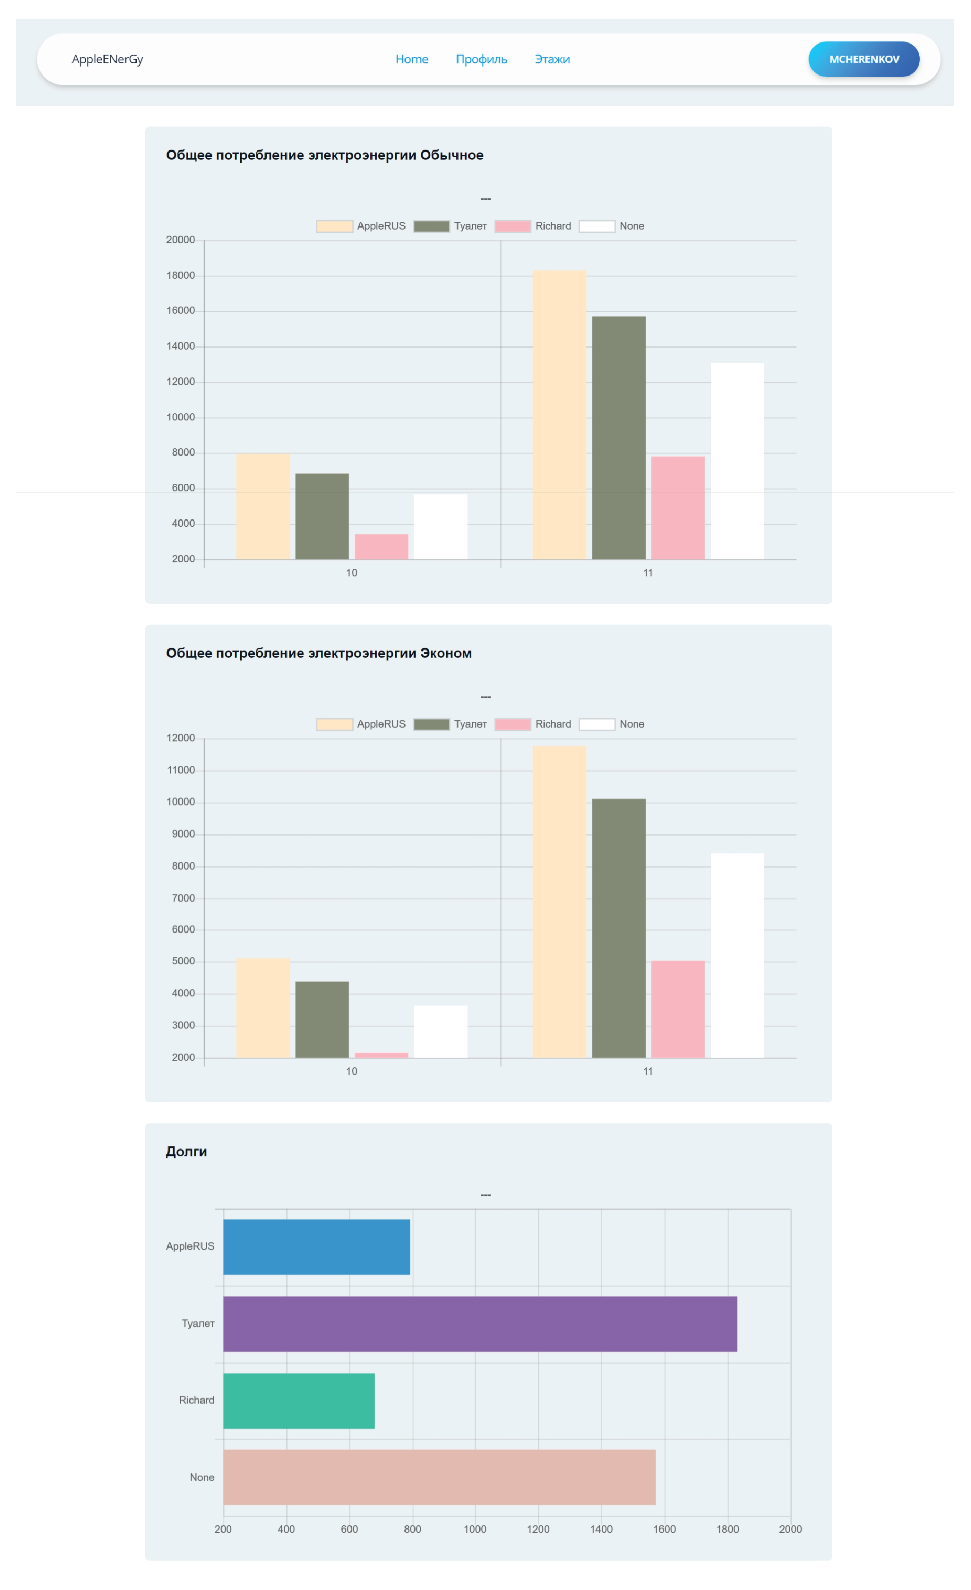
\includegraphics[width=0.65\linewidth]{templ1}
\caption{Страница с аналитикой энергопотребления в здании}
\label{templ1:image}
\end{figure}

\newpage % при необходимости можно переносить рисунок на новую страницу

\begin{figure}[ht]
	\center\includegraphics[width=0.75\linewidth]{templ2}
	\caption{Страница с аналитикой энергопотребления в здании}
	\label{templ2:image}
\end{figure}

\newpage % при необходимости можно переносить рисунок на новую страницу

\begin{figure}[ht]
	\center\includegraphics[width=0.89\linewidth]{comp}
	\caption{Концептуальная модель данных}
	\label{comp:image}
\end{figure}

%\begin{figure}[ht]
%	\includegraphics[width=1\linewidth]{comp1}
%	\caption{Концептуальная модель данных}
%	\label{comp1:image}
%\end{figure}

%\begin{figure}[ht]
%	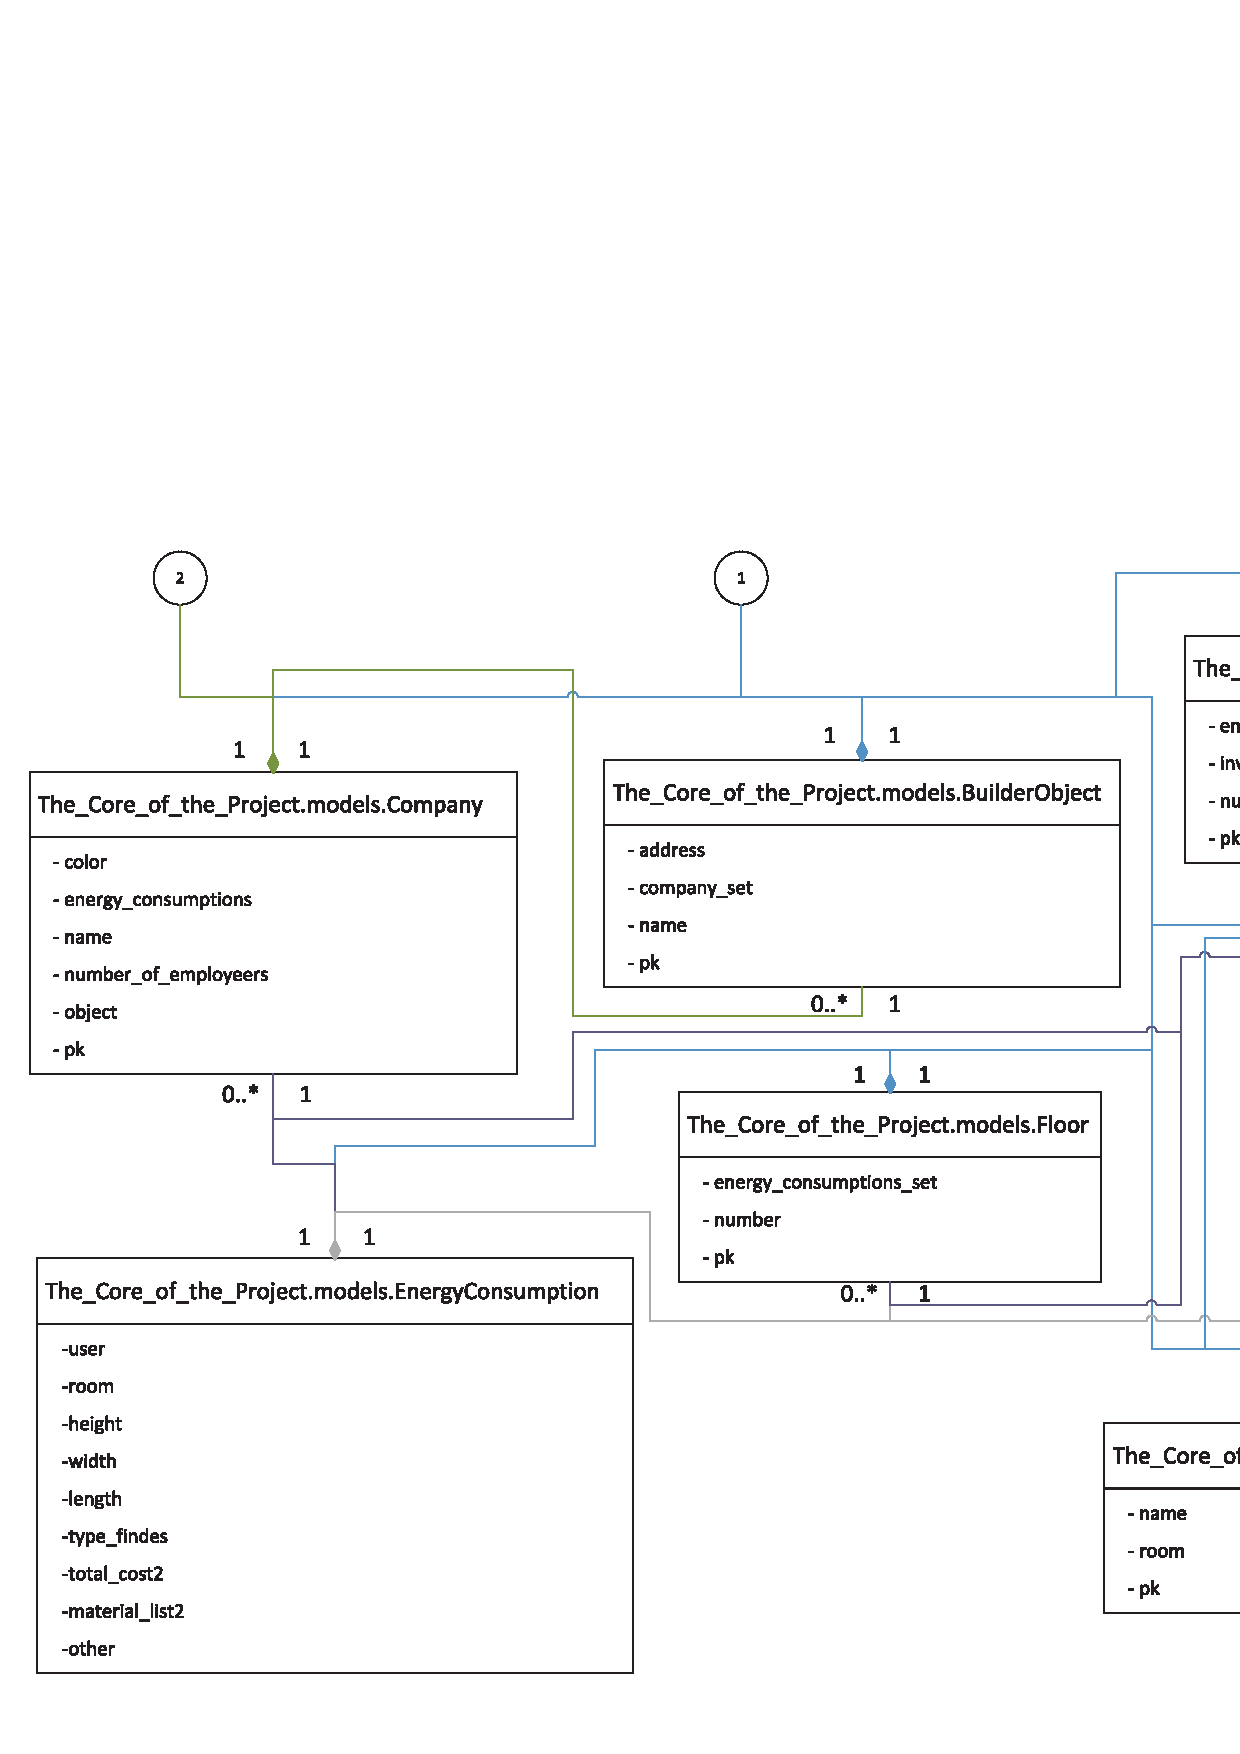
\includegraphics[width=1\linewidth]{comp2}
%	\caption{Концептуальная модель данных}
%	\label{comp2:image}
%\end{figure}

Для обеспечения удобства использования программной системы и удовлетворения потребностей пользователя, определены следующие требования к интерфейсу.

\textbf{Входные данные}

{Показания с датчиков:} Пользователь может вводить информацию о потреблении энергии вручную или автоматически, полученную от датчиков в помещениях компаний. Эти данные включают в себя значения потребления электроэнергии с и без использования умного помощника, общее количество потребляемой электроэнергии, общую стоимость потребления и данные о влажности, температуре, освещенности и наличии движения.

{Информация о помещениях, компаниях и других сущностях:} Для корректного анализа данных необходимо вводить информацию о помещениях, компаниях, этажах, предметах инвентаризации и ценах на электроэнергию.

\textbf{Выходные данные}

{Отчеты и аналитика:} Система предоставляет пользователю различные отчеты и аналитическую информацию о потреблении энергии компаниями. Эти данные включают в себя статистику по потреблению, расходам, влажности, температуре, освещенности и движению.

{Графики и визуализация:} Для наглядного представления данных система предоставляет графики и визуализацию, позволяя пользователю легко интерпретировать информацию.

{Управление данными:} Пользователь может вносить изменения в информацию о помещениях, компаниях и других сущностях через интерфейс системы.

{Оповещения:} В случае выявления аномалий или превышения установленных пороговых значений, система предоставляет уведомления и оповещения пользователю.

Система должна обеспечивать простоту ввода данных, интуитивно понятный интерфейс для взаимодействия с аналитикой, а также обеспечивать возможность быстрого доступа к ключевой информации о потреблении энергии.


%\vspace{-\figureaboveskip} % двойной отступ не нужен (можно использовать, если раздел заканчивается картинкой)

\subsection{Моделирование вариантов использования}

Для проектирования программной системы была создана модель вариантов использования. Данная модель представляет собой набор сценариев взаимодействия пользователей с системой. Диаграмма прецедентов представлена на рисунке ~\ref{precedent:image}. Она включает следующие прецеденты:

\begin{figure}[ht]
	\includegraphics[width=1\linewidth]{precedent}
	\caption{Диаграмма прецедентов}
	\label{precedent:image}
\end{figure}

{Пользовательские прецеденты:}

{\textbf{Мониторинг энергопотребления}}

\textit{Описание:} Пользователь, будучи администратором, может просматривать текущий статус энергопотребления в различных зонах здания. Эта функциональность предоставляет наглядное представление о расходе энергии и помогает выявить потенциальные проблемы.

\textit{Включает:} 
\begin{itemize}
	\item Просмотр статуса энергопотребления по зонам.
	\item Отображение графиков и диаграмм энергопотребления.
\end{itemize}

{\textbf{Настройка параметров}}

\textit{Описание:} Пользователь, имеющий права администратора, может вносить изменения в параметры системы. Это включает в себя настройку пороговых значений, оптимизацию работы системы в соответствии с текущей потребностью, и внесение изменений в режим работы оборудования.

\textit{Включает:} 
\begin{itemize}
	\item Установка пороговых значений энергопотребления.
	\item Активация/деактивация режимов работы оборудования.
	\item Регулирование параметров оптимизации энергопотребления.
\end{itemize}

{\textbf{Отчеты и аналитика}}

\textit{Описание:} Администратор системы может генерировать отчеты и аналитическую информацию о энергопотреблении. Эти отчеты предоставляют детальную статистику, позволяющую анализировать эффективность системы и выявлять тренды в потреблении энергии.

\textit{Включает:} 
\begin{itemize}
	\item Генерация отчетов по энергопотреблению за определенный период времени.
	\item Просмотр статистики по различным зонам и устройствам.
	\item Анализ трендов и предоставление рекомендаций для оптимизации.
\end{itemize}

{Системные прецеденты:}

{\textbf{Интеграция с устройствами}}

\textit{Описание:} Система должна взаимодействовать с устройствами, измеряющими энергопотребление в здании. Это включает в себя подключение к датчикам, извлечение данных и передачу команд для управления оборудованием.

\textit{Включает:} 
\begin{itemize}
	\item Подключение к датчикам энергопотребления.
	\item Извлечение данных о текущем энергопотреблении.
	\item Передача команд для регулирования работы оборудования.
\end{itemize}

{\textbf{Обработка данных}}

\textit{Описание:} Система должна обрабатывать данные, полученные от устройств, проводить анализ и формировать статистику для дальнейшего использования. Это включает в себя фильтрацию данных, выявление аномалий и расчет ключевых показателей энергопотребления.

\textit{Включает:} 
\begin{itemize}
	\item Фильтрация и агрегация данных от устройств.
	\
	
	item Анализ энергопотребления для выявления аномалий.
	\item Расчет статистических показателей для формирования отчетов.
\end{itemize}

{\textbf{Управление системой}}

\textit{Описание:} Администратор системы должен иметь возможность управлять работой системы, в том числе изменять параметры, добавлять новые устройства, и обеспечивать непрерывную работу программно-информационной системы.

\textit{Включает:} 
\begin{itemize}
	\item Добавление и удаление устройств в системе.
	\item Регулирование параметров системы для оптимальной работы.
	\item Обеспечение непрерывной работы системы и решение возможных проблем.
\end{itemize}



\subsubsection{Вариант использования <<Регистрация пользователя>>}

Заинтересованные лица и их требования: Пользователь, который не имеет учетной записи в системе, желает создать новый аккаунт.

Предусловие: Пользователь не авторизован в системе.

Постусловие: У пользователя создана учетная запись в системе.

Основной успешный сценарий:
\begin{itemize}
\item Пользователь открывает страницу регистрации.
\item Вводит свои персональные данные, такие как имя, адрес электронной почты, и пароль.
\item Нажимает кнопку "Зарегистрироваться".
\item Система проверяет валидность введенных данных.
\item В случае успешной валидации, система создает новую учетную запись пользователя.
\item Пользователю отправляется подтверждение регистрации на указанный адрес электронной почты.
\end{itemize}


\subsubsection{Вариант использования <<Регистрация компании>>}

Заинтересованные лица и их требования: Представитель компании, которая не имеет учетной записи в системе, желает зарегистрировать компанию для использования функционала системы.

Предусловие: Представитель компании не авторизован в системе.

Постусловие: В системе создана учетная запись компании, и ей назначен уникальный идентификатор.

Основной успешный сценарий:
\begin{itemize}
	\item Представитель компании открывает страницу регистрации компании.
	\item Вводит данные о компании, такие как название, цвет, расположение и количество сотрудников.
	\item Нажимает кнопку "Зарегистрировать компанию".
	\item Система проверяет валидность введенных данных.
	\item В случае успешной валидации, система создает новую учетную запись компании и присваивает ей уникальный идентификатор.
	\item Представителю компании отправляется подтверждение регистрации компании.
\end{itemize}

\subsubsection{Вариант использования <<Добавление помещения>>}

Заинтересованные лица и их требования: Пользователь (администратор), который авторизован в системе и желает добавить информацию о новом помещении.

Предусловие: Пользователь авторизован в системе и имеет доступ к функционалу управления помещениями.

Постусловие: В системе добавлена информация о новом помещении.

Основной успешный сценарий:
\begin{itemize}
	\item Пользователь переходит на страницу управления помещениями.
	\item Нажимает кнопку "Добавить помещение".
	\item Заполняет необходимые атрибуты помещения, такие как номер, площадь, этаж и прочие.
	\item Нажимает кнопку "Сохранить".
	\item Система проверяет валидность введенных данных.
	\item В случае успешной валидации, система добавляет новую информацию о помещении.
\end{itemize}

\subsubsection{Вариант использования <<Просмотр статистики по компании>>}

Заинтересованные лица и их требования: Пользователь (администратор, представитель компании), который авторизован в системе и желает получить статистическую информацию по энергопотреблению компании.

Предусловие: Пользователь авторизован в системе и имеет доступ к функционалу просмотра статистики.

Постусловие: Пользователь видит статистическую информацию по энергопотреблению компании.

Основной успешный сценарий:
\begin{itemize}
	\item Пользователь переходит на страницу статистики компании.
	\item Выбирает период, за который требуется получить статистику (например, за последний месяц).
	\item Система загружает и отображает данные о потреблении энергии компанией за выбранный период.
	\item Пользователь видит графики и диаграммы, отражающие энергопотребление, расходы и другие показатели.
\end{itemize}

\subsubsection{Вариант использования <<Просмотр статистики помещения>>}

Заинтересованные лица и их требования: Пользователь (администратор, представитель компании), который авторизован в системе и желает получить статистическую информацию по энергопотреблению определенного помещения.

Предусловие: Пользователь авторизован в системе, имеет доступ к функционалу просмотра статистики помещений и выбрал конкретное помещение.

Постусловие: Пользователь видит статистическую информацию по энергопотреблению выбранного помещения.

Основной успешный сценарий:
\begin{itemize}
	\item Пользователь переходит на страницу статистики помещения.
	\item Выбирает период, за который требуется получить статистику (например, за последний месяц).
	\item Система загружает и отображает данные о потреблении энергии выбранным помещением за выбранный период.
	\item Пользователь видит графики и диаграммы, отражающие энергопотребление, расходы и другие показатели для данного помещения.
\end{itemize}


\subsubsection{Вариант использования <<Добавление устройства>>}

Заинтересованные лица и их требования: Пользователь (администратор), который авторизован в системе и желает добавить информацию об устройстве, подключенном к определенному помещению.

Предусловие: Пользователь авторизован в системе и имеет доступ к функционалу управления устройствами помещения.

Постусловие: Информация об устройстве добавлена в систему для выбранного помещения.

Основной успешный сценарий:
\begin{itemize}
	\item Пользователь переходит на страницу управления устройствами для конкретного помещения.
	\item Выбирает опцию "Добавить устройство".
	\item Вводит информацию о новом устройстве, такую как название, тип, идентификатор, и другие характеристики.
	\item Нажимает кнопку "Добавить".
	\item Система проверяет валидность введенных данных.
	\item В случае успешной валидации, информация об устройстве добавляется к данным помещения.
	\item Пользователь видит обновленный список устройств для выбранного помещения.
\end{itemize}

\subsection{Требования к оформлению документации}

Разработка программной документации и программного изделия должна производиться согласно ГОСТ 19.102-77 и ГОСТ 34.601-90. Единая система программной документации.

\section{Технический проект}
\subsection{Общая характеристика организации решения задачи}

Для эффективного управления энергопотреблением в зданиях предлагается разработать комплексную программно-информационную систему, в основе которой лежат передовые технологии. Создаваемая система будет включать в себя несколько ключевых модулей, в том числе модули мониторинга, управления, аналитики и интеграции с внешними устройствами.

Модуль мониторинга будет ответственен за сбор и анализ данных об энергопотреблении в режиме реального времени. Это позволит системе непрерывно отслеживать изменения в расходе энергии и выявлять потенциальные области оптимизации. Модуль управления предоставит пользователям средства активного воздействия на энергопотребление, позволяя оптимизировать его в соответствии с текущими потребностями и требованиями.

Особое внимание будет уделено модулю аналитики, который обеспечит глубокий анализ данных и выделение основных трендов в потреблении энергии. Это позволит пользователям принимать информированные решения для дальнейшей оптимизации и снижения затрат. Система также будет способна интегрироваться с различными внешними устройствами и системами, обеспечивая максимальную гибкость и совместимость.

Проектная цель заключается в предоставлении пользователям возможности не только наблюдать за энергопотреблением, но и активно вмешиваться в процессы управления, с целью обеспечения оптимальной эффективности и экономии ресурсов. Разрабатываемая система ставит своей задачей создание интеллектуального и адаптивного подхода к управлению энергопотреблением, способного эффективно реагировать на изменяющиеся условия и потребности.

\subsection{Обоснование выбора технологии проектирования}

Выбор языка программирования и фреймворка - критический этап в проектировании программно-информационных систем. Для разработки системы управления энергопотреблением в зданиях был принят решительный выбор в пользу языка программирования Python с использованием фреймворка Django. Этот выбор обоснован рядом значимых преимуществ, которые существенно повысят эффективность и надежность проекта.

В первую очередь, Python предоставляет высокую степень читаемости кода и простоты синтаксиса, что облегчает понимание и совместную работу над проектом. Это особенно важно в контексте разработки программных продуктов, где четкость кода и удобство его поддержки играют ключевую роль.

Фреймворк Django, в свою очередь, предоставляет набор готовых инструментов и абстракций, спроектированных для ускорения процесса разработки. Модульность, встроенная система аутентификации, ORM (Object-Relational Mapping) для удобной работы с базой данных – все это делает Django мощным инструментом для создания сложных и надежных веб-приложений.

Дополнительно, обширное сообщество разработчиков Python и Django предоставляет широкий спектр готовых решений, библиотек и обновлений, что обеспечивает высокую поддержку и стабильность проекта на протяжении его жизненного цикла.

Такой сбалансированный выбор технологий, основанный на надежности, удобстве разработки и поддержке, позволяет ожидать успешную реализацию программно-информационной системы и обеспечивает ее легкость в последующем масштабировании и совершенствовании.

\subsubsection{Описание используемых технологий и языков программирования}

Язык программирования Python является краеугольным камнем нашего проекта, обусловленного несколькими ключевыми характеристиками. Прежде всего, простота синтаксиса Python и его высокая читаемость способствуют более эффективной разработке и сопровождению кода. Это особенно важно для проектов, направленных на веб-разработку, где четкость и легкость восприятия кода имеют первостепенное значение.

Выбор фреймворка Django обусловлен его мощью и удобством использования. Django предоставляет разработчикам набор инструментов, включая систему управления базой данных, встроенные механизмы аутентификации и авторизации, а также мощный движок для обработки URL-запросов. Это позволяет сфокусироваться на бизнес-логике приложения, ускоряя процесс разработки и повышая его надежность.

Одним из важных компонентов выбора технологии стало применение Object-Relational Mapping (ORM) в Django. ORM обеспечивает абстракцию базы данных от языка SQL, что упрощает взаимодействие с данными и позволяет разработчикам оперировать объектами в коде, а не прямо с SQL-запросами. Это не только уменьшает вероятность ошибок, связанных с базой данных, но и делает код более чистым и легко поддерживаемым.

Таким образом, выбор Python и Django, а также использование ORM, формируют сбалансированный стек технологий, обеспечивая эффективную и устойчивую основу для разработки программно-информационной системы управления энергопотреблением в зданиях.

\subsubsection{Язык программирования Python Django}

Выбор языка программирования Python с применением фреймворка Django оказался стратегически обоснованным для разработки программно-информационной системы по управлению энергопотреблением в зданиях. Этот выбор основывается на ряде ключевых преимуществ, которые содействуют эффективной и надежной реализации поставленных задач.

1. Простота и Читаемость Кода: Python славится своей простотой синтаксиса, что ускоряет процесс разработки и облегчает понимание кода. Это особенно ценно для командной работы и последующего сопровождения программы.

2. Широкое Применение в Веб-Разработке: Python является одним из наиболее популярных языков программирования в области веб-разработки. Его использование с фреймворком Django обеспечивает высокую производительность и удобство для создания сложных веб-приложений.

3. Гибкость и Мощь Django: Django предоставляет разработчикам удобные инструменты, встроенные решения и структуру проекта, что упрощает создание масштабируемых и надежных приложений. Фреймворк включает механизмы для работы с базой данных, управления пользователями, обработки форм и другие полезные функции.

4. Активное Сообщество и Поддержка: Используя Python с Django, проект получает поддержку от активного сообщества разработчиков. Это обеспечивает доступ к обширным ресурсам, библиотекам и решениям, способствуя более быстрой и безопасной разработке.

5. Объектно-Реляционное Отображение (ORM): Применение ORM в Django упрощает взаимодействие с базой данных, предоставляя абстракцию от языка SQL. Это повышает безопасность и чистоту кода, делая его более поддерживаемым.

Общий результат - это мощный и гибкий инструментарий, способствующий созданию высокоэффективной программно-информационной системы, специально нацеленной на управление энергопотреблением в зданиях.

\subsection{Диаграмма компонентов}

Диаграмма компонентов – это визуальное представление структуры программной системы, выделяя её основные компоненты и взаимосвязи между ними. Она служит инструментом для понимания архитектуры приложения.

Схема обмена данными дополняет диаграмму компонентов, демонстрируя, как информация передается между различными компонентами системы. Это важный элемент, который помогает лучше понять взаимодействие между частями приложения.

На рисунке ~\ref{compnew:image} представлена диаграмма компонентов, на которой наглядно изображены основные элементы программной системы и их взаимосвязи. 

%\begin{figure}[ht]
%	\center{\includegraphics[width=1\linewidth]{compnew}}
%	\caption{Диаграмма компонентов}
%	\label{compnew:image}
%\end{figure}


\begin{landscape}
	
	\begin{плакат}
		\includegraphics[width=0.82\linewidth]{compnew}
		\caption{Диаграмма компонентов}
		\label{compnew:image}      
	\end{плакат}
\end{landscape}

Эта визуализация позволяет разработчикам и другим участникам проекта легче ориентироваться в структуре приложения и эффективнее взаимодействовать при работе над проектом.

Каталоги:
\begin{enumerate}
\item /templates/:
\begin{itemize}
\item Описание: Содержит файлы шаблонов HTML для веб-интерфейса.
\end{itemize}

\item /static/:
\begin{itemize}
\item Описание: Хранит статические файлы, такие как CSS, JavaScript, изображения.
\end{itemize}

\end{enumerate}


Компоненты:
\begin{enumerate}
	
\item Web Interface (Веб-интерфейс)

\begin{itemize}
\item Описание: Компонент, предоставляющий пользовательский интерфейс через веб-браузер.
Файлы: templates/, static/
\end{itemize}

\item Backend Server (Серверное приложение)
\begin{itemize}
\item Описание: Компонент, обрабатывающий логику приложения и предоставляющий API для взаимодействия с фронтендом.
\item Файлы: views.py, models.py, urls.py
\end{itemize}

\item Database (База данных)
\begin{itemize}
\item Описание: Компонент, отвечающий за хранение данных.
\item Файлы: Миграции Django, models.py
\end{itemize}

\item Settings (Настройки)
\begin{itemize}
\item Описание: Компонент, содержащий настройки Django, такие как подключение к базе данных, ключи и другие конфигурационные параметры.
\item Файлы: settings.py
\end{itemize}

\item Django ORM (Объектно-реляционное отображение)
\begin{itemize}
\item Описание: Компонент, предоставляющий интерфейс для взаимодействия с базой данных через Django.
\item Файлы: Встроенные Django-модели
\end{itemize}

\item Data Reading Algorithm (Алгоритм считывания данных)
\begin{itemize}
\item Описание: Компонент, включающий алгоритмы считывания данных с устройств, таких как сенсоры, датчики влажности, температуры и другие. Отвечает за обработку данных, полученных от физических устройств, и передачу их в систему для дальнейшей обработки.
\item Файлы: {alg.py}
\end{itemize}



\end{enumerate}







%\vspace{32mm} % чтобы убрать пустую строку, которая осталась после переноса рисунка на следующую страницу
%\vspace{16mm}
%\begin{figure}[ht]
%	\center{\includegraphics[width=0.89\linewidth]{comp22}}
%	\caption{Диаграмма компонентов}
%	\label{comp22:image}
%\end{figure}

%\vspace{32mm}
%\vspace{16mm} % чтобы убрать пустую строку, которая осталась после переноса рисунка на следующую страницу


%\begin{figure}[ht]
%	\center{\includegraphics[width=0.89\linewidth]{comp33}}
%	\caption{Диаграмма компонентов}
%	\label{comp33:image}
%\end{figure}
%\vspace{-8mm} % чтобы убрать пустую строку, которая осталась после переноса рисунка на следующую страницу


\begin{comment}

На диаграмме компонентов выделены следующие основные компоненты views.py:
\begin{itemize}
\item \textbf{home} - Обработчик отображения домашней страницы.

Parameters:
- request: объект запроса Django.

Returns:
- Получает данные о текущем пользователе из запроса.
- Формирует контекст с данными о пользователе.
- Возвращает страницу домашней страницы с переданным контекстом.

Возвращаемый шаблон:
- 'AC/Home/home-ac.html'.

Контекст:
- 'user': Объект текущего пользователя.

\item \textbf{create-company} - Обработчик создания новой компании.

Parameters:
- request: объект запроса Django.

Returns:
- Если метод запроса POST:
- Получает данные из формы создания компании.
- Если форма валидна, сохраняет новую компанию.
- Перенаправляет на домашнюю страницу.
- Если метод запроса GET:
- Создает форму для создания компании.
- Возвращает страницу с формой создания компании.

Возвращаемый шаблон:
- Если метод запроса GET или POST:
- 'AC/Admin/add-company-ac.html'.

Контекст:
- 'form': Экземпляр формы создания компании.

\item \textbf{delete-company} - Обработчик удаления компании.

Parameters:
- request: объект запроса Django.
- company-id: идентификатор компании, которую нужно удалить.

Returns:
- При успешном удалении компании:
- Перенаправляет пользователя на домашнюю страницу.
- Если компания не найдена:
- Возвращает страницу с ошибкой 404.


\item \textbf{create-object} - Обработчик создания нового объекта.

Parameters:
- request: объект запроса Django.

Returns:
- Если метод запроса POST:
- Получает данные из формы создания объекта.
- Если форма валидна, сохраняет новый объект.
- Перенаправляет на домашнюю страницу.
- Если метод запроса GET:
- Создает форму для создания объекта.
- Возвращает страницу с формой создания объекта.

Возвращаемый шаблон:
- Если метод запроса GET или POST:
- 'AC/Admin/add-object-ac.html'.

Контекст:
- 'form': Экземпляр формы создания объекта.

\item \textbf{create-object-to-room} - Обработчик создания нового объекта в комнате.

Parameters:
- request: объект запроса Django.

Returns:
- Если метод запроса POST:
- Получает данные из формы создания объекта в комнате.
- Если форма валидна, сохраняет новый объект в комнате.
- Перенаправляет на домашнюю страницу.
- Если метод запроса GET:
- Создает форму для создания объекта в комнате.
- Возвращает страницу с формой создания объекта в комнате.

Возвращаемый шаблон:
- Если метод запроса GET или POST:
- 'AC/Admin/add-object-to-room-ac.html'.

Контекст:
- 'form': Экземпляр формы создания объекта в комнате.


\item \textbf{create-room} - Обработчик создания новой комнаты.

Parameters:
- request: объект запроса Django.

Returns:
- Если метод запроса POST:
- Получает данные из формы создания комнаты.
- Если форма валидна, сохраняет новую комнату.
- Перенаправляет на домашнюю страницу.
- Если метод запроса GET:
- Создает форму для создания комнаты.
- Возвращает страницу с формой создания комнаты.

Возвращаемый шаблон:
- Если метод запроса GET или POST:
- 'AC/Admin/add-room-ac.html'.

Контекст:
- 'form': Экземпляр формы создания комнаты.

\item \textbf{profile} -Обработчик отображения профиля пользователя.

Parameters:
- request: объект запроса Django.

Returns:
- Получает данные пользователя по его идентификатору из запроса.
- Формирует контекст с данными пользователя.
- Возвращает страницу профиля с переданным контекстом.

Возвращаемый шаблон:
- 'AC/Profile/profile-ac.html'.

Контекст:
- 'user': Объект пользователя с данными профиля.

\item \textbf{update-profile} -  Обработчик обновления профиля пользователя.

Parameters:
- request: объект запроса Django.

Returns:
- Если метод запроса POST:
- Получает данные из формы обновления профиля пользователя.
- Если форма валидна, сохраняет обновленные данные профиля.
- Перенаправляет на страницу профиля.
- Если метод запроса GET:
- Создает форму для редактирования профиля с данными текущего пользователя.
- Возвращает страницу с формой редактирования профиля.

Возвращаемый шаблон:
- Если метод запроса GET или POST:
- 'AC/Profile/edit-profile-ac.html'.

Контекст:
- Если метод запроса GET:
- 'form': Экземпляр формы редактирования профиля с данными текущего пользователя.

\item \textbf{change-password} - Обработчик изменения пароля пользователя.

Parameters:
- request: объект запроса Django.

Returns:
- Если метод запроса POST:
- Получает новый пароль из формы.
- Устанавливает новый пароль для текущего пользователя.
- Сохраняет изменения и обновляет хэш аутентификации в сессии.
- Перенаправляет на страницу профиля.
- Если метод запроса GET:
- Возвращает страницу с формой изменения пароля.

Возвращаемый шаблон:
- Если метод запроса GET или POST:
- 'AC/Profile/forgotyourpassword-ac.html'.

\item \textbf{reset-password} -     Обработчик сброса пароля пользователя.

Parameters:
- request: объект запроса Django.

Returns:
- Если метод запроса POST:
- Получает имя пользователя из формы.
- Пытается найти пользователя с указанным именем.
- Если пользователь найден, устанавливает новый пароль 'qwerty123' и сохраняет изменения.
- Перенаправляет на страницу входа.
- Если пользователь с указанным именем не найден, обработывает исключение User.DoesNotExist.
- Если метод запроса GET:
- Возвращает страницу сброса пароля.

Возвращаемый шаблон:
- Если метод запроса GET:
- 'AC/Profile/forgotyourpassword-ac.html'.
- Если метод запроса POST:
- Нет.

\item \textbf{delete-profile} - Обработчик удаления профиля пользователя.

Parameters:
- request: объект запроса Django.

Returns:
- Если метод запроса POST:
- Получает текущего пользователя.
- Удаляет профиль пользователя.
- Выполняет выход пользователя из системы.
- Перенаправляет на страницу входа.
- Если метод запроса GET:
- Возвращает страницу подтверждения удаления профиля.

Возвращаемый шаблон:
- Если метод запроса GET:
- 'AC/Profile/delete-profile-ac.html'.
- Если метод запроса POST:
- Нет.

\item \textbf{register} - Обработчик регистрации пользователей.

Parameters:
- request: объект запроса Django.

Returns:
- Если метод запроса POST:
- Если данные формы валидны, создается новый пользователь с использованием данных из формы.
- Выполняется вход в систему от имени нового пользователя.
- Перенаправляет на страницу профиля.
- Если метод запроса GET:
- Создает экземпляр формы регистрации.
- Рендерит страницу регистрации с пустой формой.

Возвращаемый шаблон:
- 'AC/Profile/registration-ac.html'

Контекст:
- 'form': Экземпляр формы регистрации.

\item \textbf{login-view} - Обработчик входа пользователя в систему.

Parameters:
- request: объект запроса Django.

Returns:
- Если метод запроса POST:
- Проверяет переданные учетные данные пользователя с использованием Django's authentication system.
- Если учетные данные верны, выполняет вход пользователя в систему и перенаправляет на страницу профиля.
- В противном случае, возвращает страницу входа с сообщением об ошибке.
- Если метод запроса GET:
- Возвращает страницу входа.

Возвращаемый шаблон:
- Если метод запроса POST и учетные данные неверны:
- 'AC/Profile/login-ac.html' с переданным сообщением об ошибке.
- В остальных случаях:
- 'AC/Profile/login-ac.html'.

Контекст:
- Если метод запроса POST и учетные данные неверны:
- 'error-message': Сообщение об ошибке для отображения на странице входа.

\item \textbf{logout-view} - Обработчик выхода пользователя из системы.

Parameters:
- request: объект запроса Django.

Returns:
- Выполняет выход текущего пользователя из системы.
- Перенаправляет на страницу входа.

\item \textbf{floor-view} - Обработчик отображения этажа с комнатами.

Parameters:
- request: объект запроса Django.

Returns:
- Получает номер этажа из параметра запроса или устанавливает значение по умолчанию (1).
- Вычисляет предыдущий и следующий этажи.
- Пытается получить объект этажа по номеру.
- Если объект этажа существует, получает комнаты на этом этаже.
- Формирует контекст с данными о текущем этаже, предыдущем и следующем этажах, а также списком комнат.
- Возвращает страницу с информацией об этаже и комнатах или страницу ошибки 404, если этаж не найден.

Возвращаемый шаблон:
- Если этаж найден:
- 'AC/floors.html'.
- Если этаж не найден:
- 'AC/404.html'.

\item \textbf{energy-consumption-chart} -     Получение данных о потреблении энергии для компании.

Parameters:
- company-id: Идентификатор компании.

Returns:
- months: Список месяцев.
- consumption-without-assistant: Суммарное потребление электроэнергии без использования умного помощника.
- consumption-with-assistant: Суммарное потребление электроэнергии с использованием умного помощника.


\item \textbf{cabinet-view} -     Обработчик отображения информации о кабинете (комнате).

Parameters:
- request: объект запроса Django.
- floor: Номер этажа.
- cab-num: Номер кабинета.

Returns:
- Если кабинет найден:
- Получает данные о кабинете, инвентаризации и потреблении энергии.
- Формирует контекст с данными о кабинете, предыдущем и следующем кабинетах, месяцах и потреблении энергии.
- Возвращает страницу с информацией о кабинете.
- Если кабинет не найден:
- Возвращает страницу ошибки 404.


\item \textbf{dashboard-sensors-view} - Обработчик отображения данных по датчикам и потреблению энергии для определенной компании и комнаты в определенную дату.

Parameters:
- request: объект запроса Django.
- company: Идентификатор компании (предприятия).
- room: Идентификатор комнаты.

Returns:
- Если данные существуют для указанной компании, комнаты и даты:
- Получает данные из модели EnergyConsumption.
- Формирует контекст с полученными данными и предыдущей и следующей датами.
- Возвращает страницу с отображением данных по датчикам и потреблению энергии.
- Если данных не существует:
- Возвращает страницу ошибки 404.

Возвращаемый шаблон:
- 'AC/dashboard-sensors.html' в случае успешного нахождения данных.
- 'AC/404.html' в случае отсутствия данных.

Контекст:
- 'id': Идентификатор записи.
- 'company': Компания (предприятие).
- 'room': Комната.
- 'date': Дата.
- 'consumption-without-an-assistant': Потребление энергии без использования умного помощника.
- 'consumption-with-an-assistant': Потребление энергии с использованием умного помощника.
- 'total-amount-of-electricity-consumed-without-an-assistant': Общее потребление электроэнергии без использования умного помощника.
- 'total-amount-of-electricity-consumed-with-the-assistant': Общее потребление электроэнергии с использованием умного помощника.
- 'total-cost-without-an-assistant': Общая стоимость электроэнергии без использования умного помощника.
- 'total-cost-with-an-assistant': Общая стоимость электроэнергии с использованием умного помощника.
- 'humidity': Влажность.
- 'temperature': Температура.
- 'illumination': Освещенность.
- 'motion': Наличие движения.
- 'prev-date': Предыдущая дата.
- 'next-date': Следующая дата.

\end{itemize}

\end{comment}


\subsubsection{Описание настройки Django}

Настройка Django в проекте осуществляется через два ключевых файла: settings.py и urls.py. В этих файлах определена конфигурация приложения, включая параметры базы данных, пути к шаблонам, обработку статических файлов и другие настройки. В settings.py размещаются параметры, определяющие общую конфигурацию проекта, такие как настройки базы данных, приложения, подключение статических и медиа файлов, а также многое другое. С другой стороны, в urls.py определяются пути маршрутизации, которые связывают URL-адреса с соответствующими представлениями и функциональностью приложения. Эти два файла играют ключевую роль в формировании и управлении всеми аспектами функционирования Django-приложения, обеспечивая его корректное взаимодействие с веб-сервером и клиентскими запросами.
 
\paragraph{База данных}

Один из важных аспектов Django-проекта – это выбор и настройка системы управления базами данных (СУБД). В данном случае, в качестве СУБД используется PostgreSQL, предоставляющая надежное и мощное хранилище данных.

Для интеграции PostgreSQL в Django проект, первоначально необходимо установить соответствующий пакет драйвера, в данном случае, psycopg2. Этот драйвер обеспечивает связь между Django и PostgreSQL, обеспечивая эффективное взаимодействие с базой данных.

После установки драйвера, производится конфигурация подключения к базе данных в файле settings.py. Здесь определяются параметры, такие как имя базы данных, пользователь, пароль, хост и порт, необходимые для успешного соединения с PostgreSQL. Это обеспечивает правильную интеграцию между Django приложением и выбранной базой данных, что является фундаментом для эффективного хранения и обработки данных в рамках проекта. Пример настройки:

 
\begin{lstlisting}[language=Python]
DATABASES = {
	'default': {
		'ENGINE': 'django.db.backends.postgresql',
		'NAME': 'mydatabase',
		'USER': 'mcherenkov',
		'PASSWORD': '*2nm(h(tIs2u4AJ#',
		'HOST': 'localhost',
		'PORT': '5432',
	}
}
\end{lstlisting}  
 
Эти параметры включают в себя имя базы данных, пользователя, пароль, хост и порт для подключения к PostgreSQL.

\paragraph{Статические файлы и медиа}

Настройки для обработки статических файлов и медиа файлов (например, изображений, загружаемых пользователями) также определены в settings.py. Важным аспектом конфигурации Django-проекта является определение параметров обработки статических и медиа файлов. Эти файлы могут включать в себя стили, скрипты, изображения, а также медиа-контент, загружаемый пользователями.
 
Такие настройки позволяют эффективно управлять статическими и медиа-ресурсами в Django-проекте, обеспечивая их доступность и корректное отображение на веб-страницах.Пример настроек для статических файлов:
 
\begin{lstlisting}[language=Python]
STATIC_URL = '/static/'
STATICFILES_DIRS = [BASE_DIR / "static"]

MEDIA_URL = '/media/'
MEDIA_ROOT = BASE_DIR / "media"

\end{lstlisting}  

Здесь STATIC-URL указывает префикс для статических файлов, а STATICFILES-DIRS - на каталог, где хранятся эти файлы.

MEDIA-URL и MEDIA-ROOT аналогичны, но используются для обработки медиа файлов.

\paragraph{Настройки безопасности}

Django также предоставляет настройки безопасности, такие как секретный ключ, список разрешенных хостов (ALLOWED-HOSTS), и другие параметры. Пример:

 
\begin{lstlisting}[language=Python]
SECRET_KEY = 'django-insecure-b)te6480y4j&yunr@zy6v#$2u(r@06q3kb$m@=d1n!_8t&(xj!'
DEBUG = False
ALLOWED_HOSTS = ['mcherenkov.com']
\end{lstlisting} 
 
Секретный ключ должен быть уникальным и долгим случайным значением. Включение параметра DEBUG в режиме разработки может быть удобным для поиска ошибок, но необходимо отключить его в продакшн окружении. Список разрешенных хостов (ALLOWED-HOSTS) определяет, какие хосты могут обращаться к вашему серверу. 

 
\subsection{Диаграмма размещения}
\begin{comment}
	

Для создания диаграммы размещения, нам нужно учитывать архитектурные компоненты программной системы и то, как они будут размещены на физических устройствах. Ниже представлен пример общей структуры диаграммы размещения для "Программно-информационная система для управления энергопотреблением в зданиях". В диаграмме должны быть представлены следующие элементы:
\end{comment}

При проектировании диаграммы размещения необходимо тщательно рассмотреть взаимодействие архитектурных компонентов программной системы и их распределение по физическим устройствам. Эффективное размещение данных компонентов определяет стабильность и производительность системы. Приведенный ниже пример диаграммы размещения является иллюстрацией общей структуры "Программно-информационной системы для управления энергопотреблением в зданиях", включающей в себя ключевые элементы, начиная от клиентских устройств и заканчивая устройствами управления энергопотреблением в физических зданиях.

Серверная инфраструктура, показывает сервера, на которых размещаются серверные компоненты системы, такие как веб-сервер, базы данных и другие серверные приложения.


\begin{landscape}
	
	\begin{плакат}
		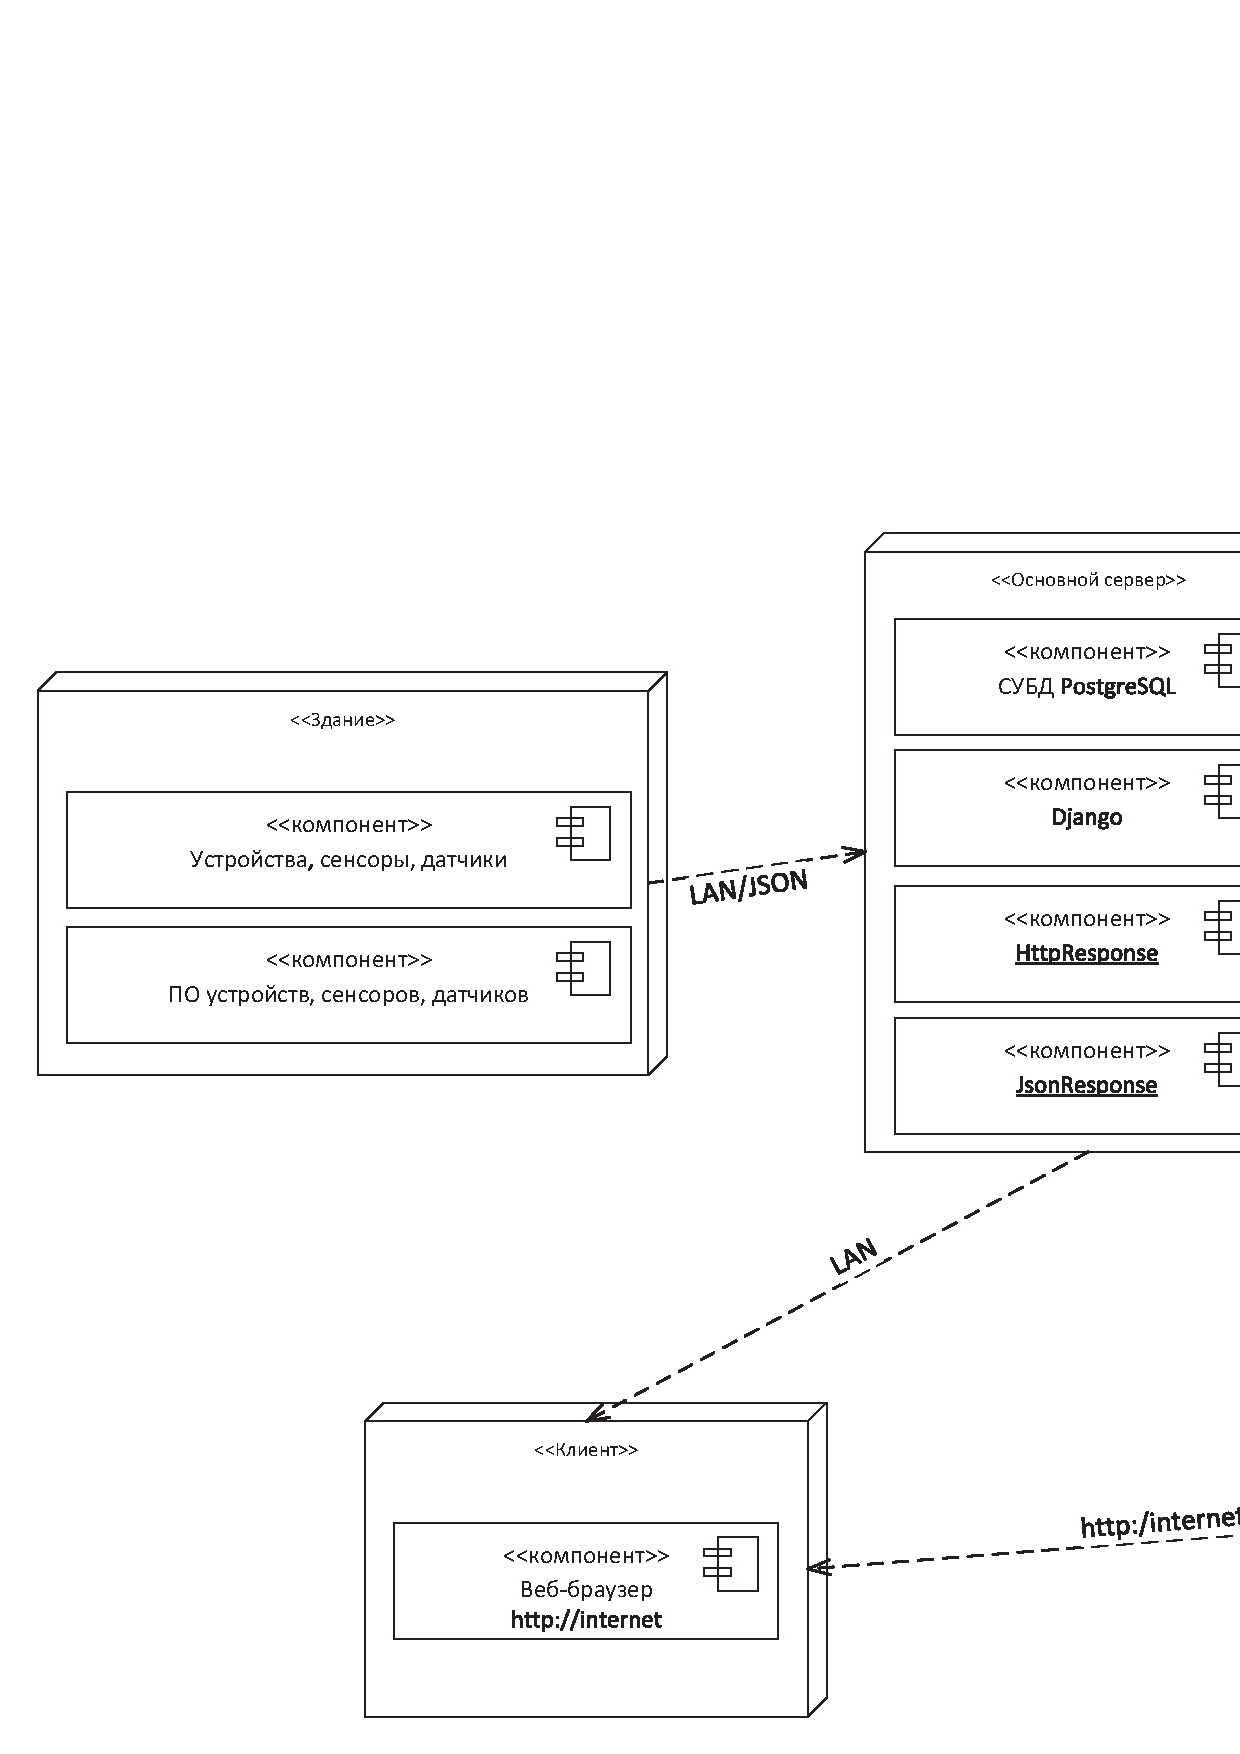
\includegraphics[width=0.82\linewidth]{place}
		\caption{Диаграмма размещения}
		\label{place:image}      
	\end{плакат}
\end{landscape}



\begin{enumerate}


\item {Сервер:}
\begin{itemize}
	\item {Описание:} Физический или виртуальный сервер, на котором размещена программно-информационная система. Сервер выполняет обработку запросов, взаимодействует с базой данных, и управляет основной логикой системы.
	\item {Размещение:} Сервер расположен в дата-центре компании и подключен к высокоскоростной сети интернета.
	\item {Компоненты:} Django приложение, бизнес-логика, веб-сервер.
\end{itemize}

\item {База данных:}
\begin{itemize}
	\item {Описание:} Хранилище данных, где сохраняются все необходимые для системы информационные записи. В данной системе используется реляционная база данных для хранения данных о компаниях, потреблении энергии, настройках и других сущностях.
	\item {Размещение:} Физически база данных размещена на сервере в дата-центре, обеспечивая быстрый доступ к данным.
	\item {Компоненты:} PostgreSQL (или другая СУБД), таблицы с данными.
\end{itemize}

\item Устройства сбора данных:
\begin{itemize}
\item  {Описание:} Физические устройства, установленные в зданиях, ответственные за сбор данных о потреблении энергии и внесение корректив в управление энергопотреблением в реальном времени. Компоненты включают в себя сенсоры, датчики влажности, температуры, освещенности и другие.
\item  {Размещение:} Сенсоры и датчики подключены к локальной сети в каждом здании компании, обеспечивая сбор данных в реальном времени.
\item  {Компоненты:} Сенсоры, датчики, средства сбора и передачи данных.
\item  {Сеть:} Устройства сбора данных подключены к локальной сети здания, обеспечивая передачу данных на сервер через сетевой протокол (например, TCP/IP). Данные могут быть переданы в формате JSON для удобства обработки на сервере.
\end{itemize}
	
\item Пользовательские устройства():
\begin{itemize}
	\item {Описание:} Пользовательские интерфейсы представлены на клиентских устройствах, таких как компьютеры, планшеты или мобильные устройства. Здесь пользователи могут взаимодействовать с системой, вводя данные или получая информацию.
	\item {Размещение:} Устройства клиентов находятся в офисах компаний, а также могут использоваться удаленные рабочие места.
	\item {Компоненты:} Браузеры (Google Chrome, Mozilla Firefox, Safari и др.), интерфейс пользователя.
\end{itemize}


\item Сетевые соединения, стрелки, обозначающие сетевые соединения между устройствами, чтобы показать, как данные передаются между ними.


\end{enumerate}

Диаграмма размещения демонстрирует (рис.~\ref{place:image}) , как каждый компонент системы взаимодействует друг с другом и как данные передаются между устройствами.


%\vspace{-8mm} % чтобы убрать пустую строку, которая осталась после переноса рисунка на следующую страницу
%\begin{figure}[ht]
%	\center{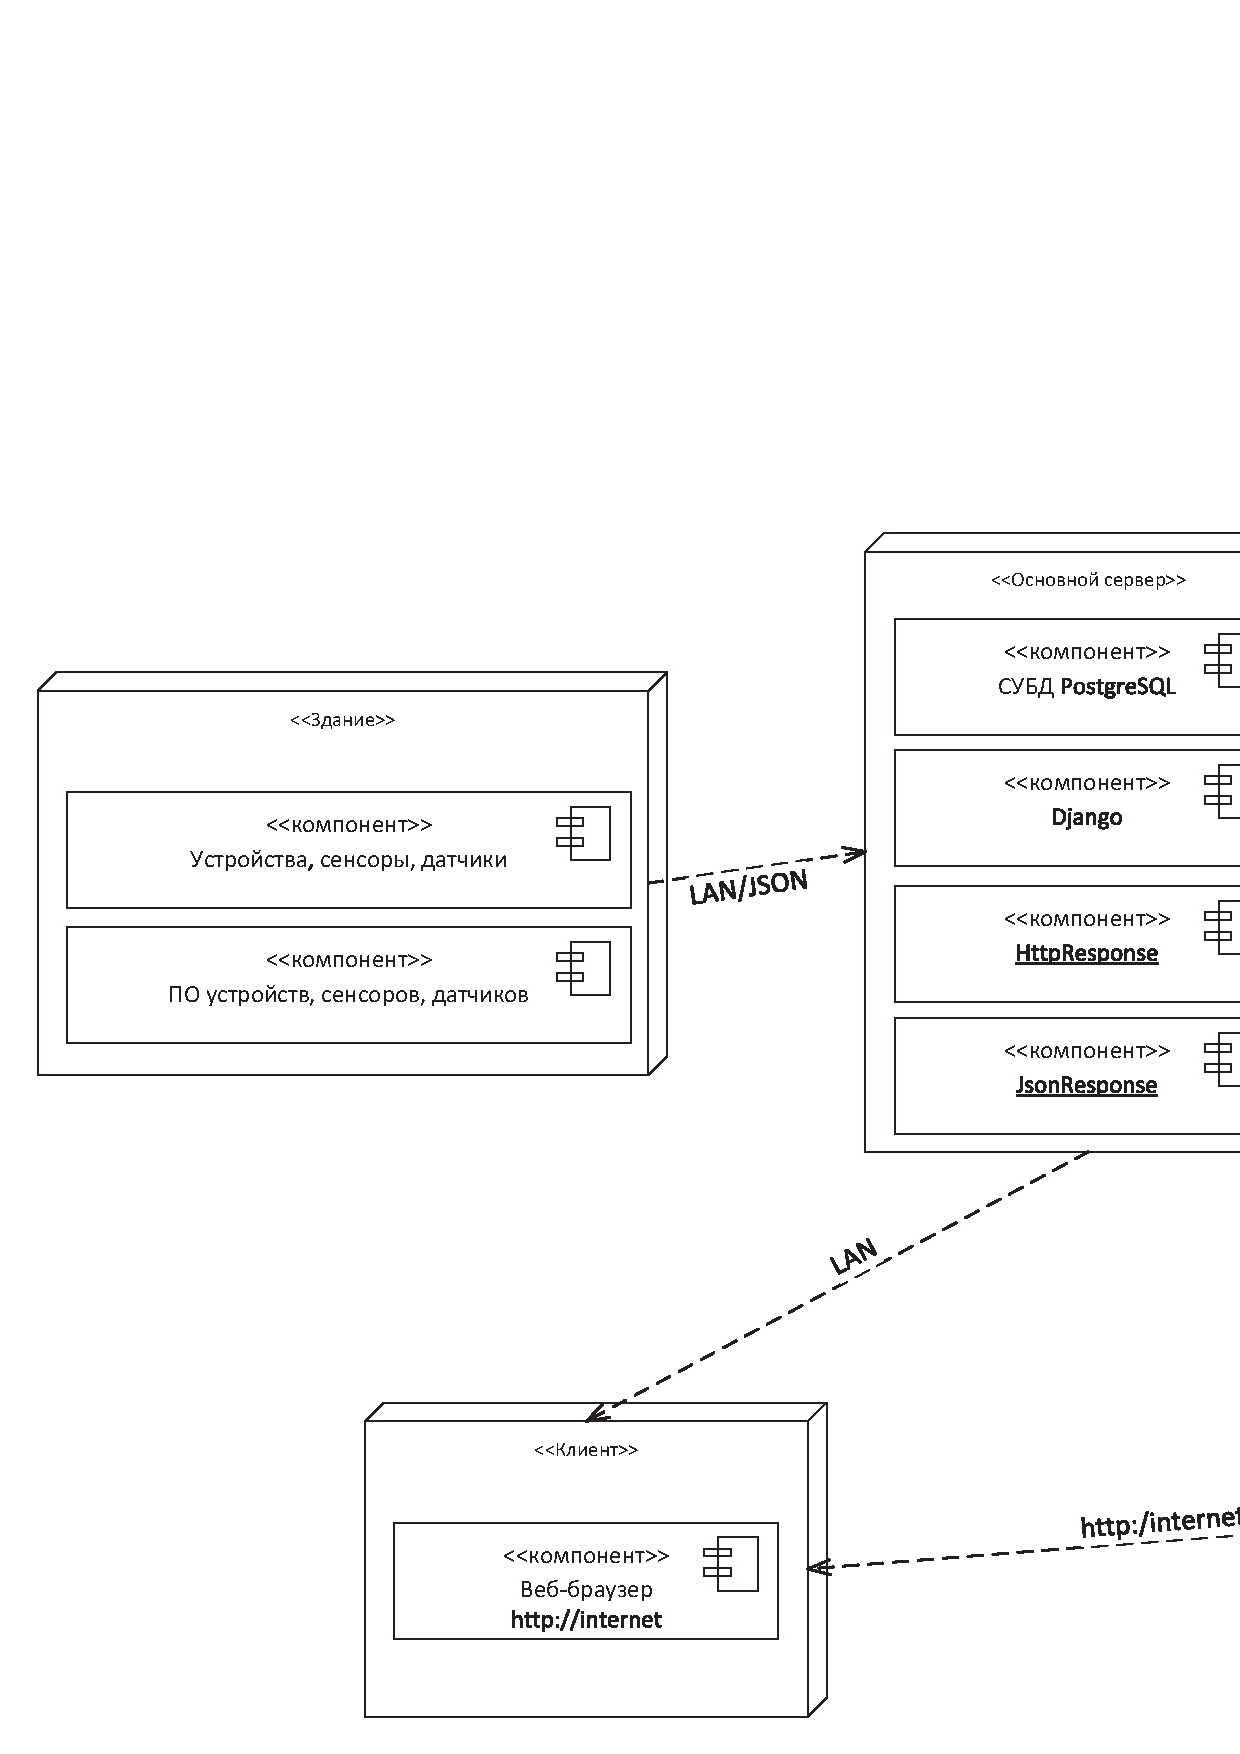
\includegraphics[width=0.9\linewidth]{place}}
%	\caption{Диаграмма размещения}
%	\label{place:image}
%\end{figure}



\subsection{Диаграмма классов}

Диаграмма классов представляет собой визуализацию структуры классов программной системы и их взаимосвязей. Ниже приведено описание основных классов системы "Программно-информационная система для управления энергопотреблением в зданиях".

Классы, представление классов с их атрибутами и методами:

\begin{enumerate}
	
\item {Класс <<EnergyConsumption>>:} Модель для учета потребленной энергии.
\begin{itemize}
	\item {Атрибуты:}  company, room, floor, date, consumption\_without\_an\_assistant, consumption\_with\_an\_assistant, total\_amount\_of\_electricity\_consumed\_without\_an\_assistant, total\_amount\_of \_electricity\_consumed\_with\_the\_assistant, total\_cost\_without\_an\_assistant, total\_cost\_with\_an\_assistant, humidity, temperature, illumination, motion.
	\item {Методы:} {\_\_str\_\_}.
\end{itemize}

\item {Класс <<InventoryItemsNumber>>:} Модель для представления предметов в помещении.
\begin{itemize}
	\item {Атрибуты:} name, room.
	\item {Методы:} \_\_str\_\_.
\end{itemize}

\item {Класс <<Company>>:} Модель для представления компаний.
\begin{itemize}
	\item {Атрибуты:} name, color, object, number-of-employees.
	\item {Методы:} \_\_str\_\_.
\end{itemize}

\item {Класс <<Floor>>:} Модель для представления этажей.
\begin{itemize}
	\item {Атрибуты:} number.
	\item {Методы:} \_\_str\_\_.
\end{itemize}

\item {Класс <<Electricity>>:} Модель для представления электроэнергии.
\begin{itemize}
	\item {Атрибуты:} price, volume.
	\item {Методы:} \_\_str\_\_.
\end{itemize}
\end{enumerate}

{Объяснение основных классов:}

\begin{itemize}
	
	\item {EnergyConsumption:} Этот класс предназначен для учета и хранения данных о потреблении энергии в зданиях. Атрибуты класса включают в себя информацию о компании, помещении, этаже, дате, количестве потребленной энергии с и без использования системы управления, общей стоимости, а также дополнительные параметры, такие как влажность, температура, освещенность и обнаружение движения.
	
	\item {Класс <<InventoryItemsNumber>>:} Данный класс предназначен для представления предметов, находящихся в конкретном помещении. Атрибуты класса включают в себя название предмета и ссылку на помещение, где он находится. 
	
	\item {Класс <<Company>>:} Этот класс используется для представления компаний, использующих систему управления энергопотреблением. Атрибуты класса включают в себя название компании, цвет для визуализации, тип объекта компании и количество сотрудников.
	
	\item {Класс <<Floor>>:} Класс предназначен для хранения информации об этажах здания. Атрибуты класса включают в себя номер этажа.
	
	\item {Класс <<Electricity>>:} Данный класс используется для представления электроэнергии, собираемой и потребляемой системой. Атрибуты класса включают в себя цену за единицу электроэнергии и объем потребленной энергии.

\end{itemize}

Диаграмма классов представлена на рисунке ~\ref{classd111:image}, представляющее основные модели данных в вашем проекте на Django.


%Диаграмма классов представлена на рисунках ~\ref{classd1:image} - ~\ref{classd2:image}, %представляющая основные модели данных в вашем проекте на Django.

%\begin{figure}[ht]
%	\center{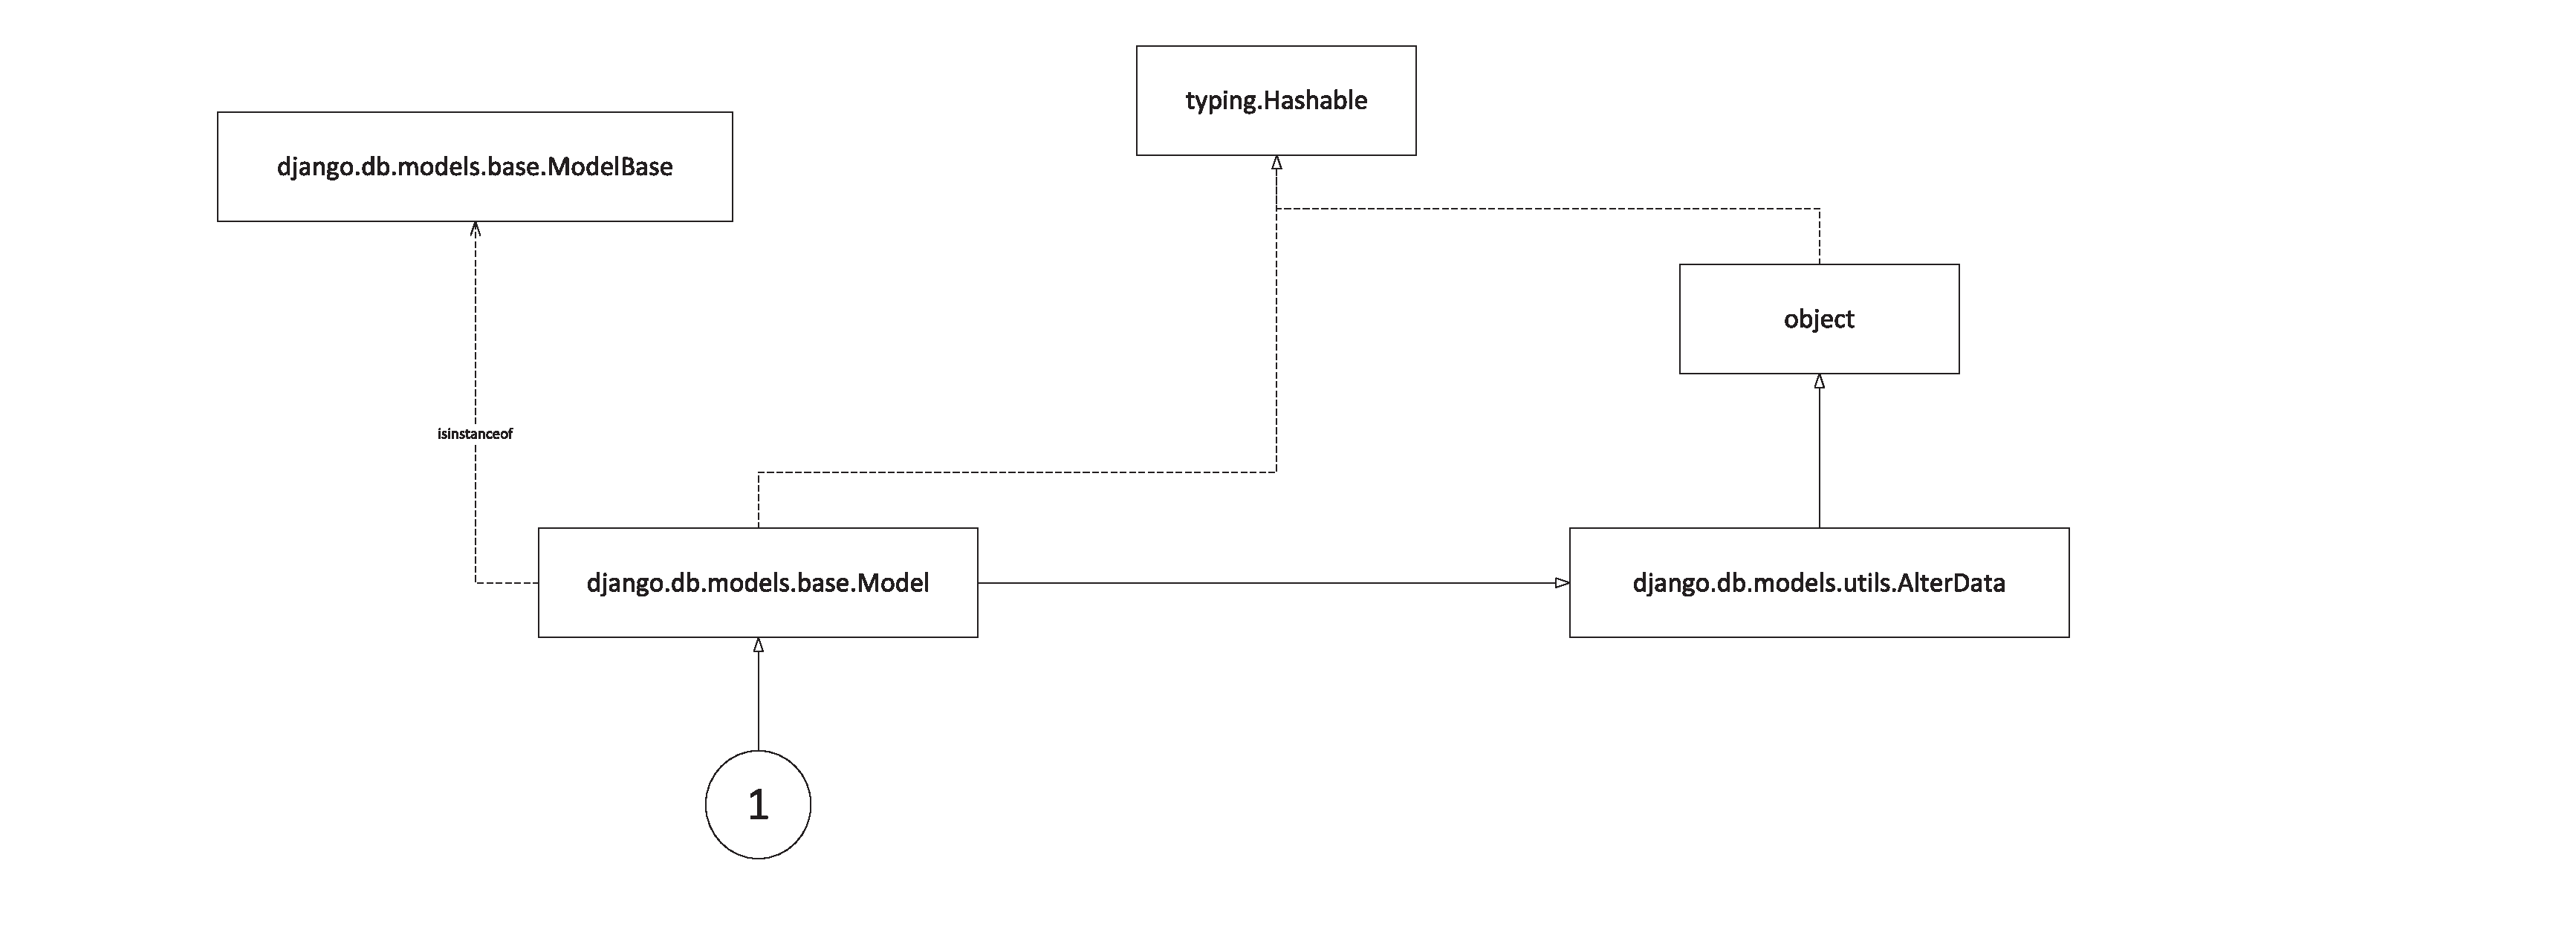
\includegraphics[width=1\linewidth]{classd1}}
%	\caption{Диаграмма классов}
%	\label{classd1:image}
%\end{figure}

%\newpage

%\begin{figure}[ht]
%	\center{\includegraphics[width=0.9\linewidth]{classd2}}
%	\caption{Диаграмма классов}
%	\label{classd2:image}
%\end{figure}


\begin{landscape}
	
	\begin{плакат}
		\includegraphics[width=0.82\linewidth]{classd111}
		\caption{Диаграмма классов}
		\label{classd111:image}      
	\end{плакат}
\end{landscape}



\newpage

\subsection{Содержание информационных блоков. Основные сущности}

Проанализировав требования, можно выделить несколько основных сущностей:

\begin{itemize}
	\item "<Потребление энергии">;
	\item "<Помещения">;
	\item "<Компании">;
	\item "<Этажи">;
	\item "<Предметы инвентаризации">;
	\item "<Электроэнергия">.
\end{itemize}

Сущность, отражающая данные о потреблении энергии компаниями на различных этажах и в разных помещениях. В состав сущности "<Потребление энергии"> можно включить атрибуты, представленные в таблице \ref{potrenergy:table}.

\begin{xltabular}{\textwidth}{|p{4cm}|l|p{1.7cm}|X|}
	\caption{Атрибуты сущности "<Потребление энергии">\label{potrenergy:table}}\\ \hline
	\centrow Поле & \centrow Тип & \centrow Обяза\-тельное & \centrow Описание \\ \hline
	\endfirsthead
	\continuecaption{Продолжение таблицы \ref{potrenergy:table}}
	\centrow Поле & \centrow Тип & \centrow Обяза\-тельное & \centrow Описание \\ \hline
	\finishhead
	company & ForeignKey(Company) & Да & Компания, потребляющая энергию. \\ \hline
	room & ForeignKey(Room) & Нет & Помещение, в котором измеряется потребление. \\ \hline
	floor & ForeignKey(Floor) & Нет & Этаж, на котором расположено помещение. \\ \hline
	date & DateField & Да & Дата, когда было измерено потребление. \\ \hline
	consumption-without-an-assistant & JSONField & Да & Потребление электроэнергии без использования умного помощника. \\ \hline
	consumption-with-an-assistant & JSONField & Да & Потребление электроэнергии с использованием умного помощника. \\ \hline
	total-amount-without-an-assistant & FloatField & Да & Общее количество потребляемой электричества без использования помощника. \\ \hline
	total-amount-with-the-assistant & FloatField & Да & Общее количество электричества, потребляемого с использованием помощника. \\ \hline
	total-cost-without-an-assistant & JSONField & Да & Общая стоимость потребления без использования помощника.\\ \hline
	total-cost-with-an-assistant & JSONField & Да & Общая стоимость потребления с использованием помощника. \\ \hline
	humidity & JSONField & Да & Значение влажности.\\ \hline
	temperature & JSONField & Да & Значение температуры. \\ \hline
	illumination & JSONField & Да & Значение освещенности.\\ \hline
	motion & JSONField & Да & Наличие движения.
\end{xltabular}
 
Сущность, описывающая различные помещения на этажах компаний. В состав сущности "<Помещения"> можно включить атрибуты, представленные в таблице \ref{room:table}.

\begin{xltabular}{\textwidth}{|p{4cm}|l|p{1.7cm}|X|}
	\caption{Атрибуты сущности "<Помещения">\label{room:table}}\\ \hline
	\centrow Поле & \centrow Тип & \centrow Обяза\-тельное & \centrow Описание \\ \hline
	\endfirsthead
	\continuecaption{Продолжение таблицы \ref{room:table}}
	\centrow Поле & \centrow Тип & \centrow Обяза\-тельное & \centrow Описание \\ \hline
	\finishhead
		name & CharField & Да & Название помещения.\\ \hline
		floor & ForeignKey(Floor) & Да & Этаж, на котором расположено помещение.
\end{xltabular}
 
Сущность, представляющая информацию о компаниях, потребляющих энергию. В состав сущности "<Компании"> можно включить атрибуты, представленные в таблице \ref{company:table}.

\begin{xltabular}{\textwidth}{|p{4cm}|l|p{1.7cm}|X|}
	\caption{Атрибуты сущности "<Компании">\label{company:table}}\\ \hline
	\centrow Поле & \centrow Тип & \centrow Обяза\-тельное & \centrow Описание \\ \hline
	\endfirsthead
	\continuecaption{Продолжение таблицы \ref{company:table}}
	\centrow Поле & \centrow Тип & \centrow Обяза\-тельное & \centrow Описание \\ \hline
	\finishhead
		name & CharField & Да & Название компании.\\ \hline
		color & ForeignKey(Color) & Нет & Цвет, ассоциированный с компанией.\\ \hline
		object & ForeignKey(BuilderObject) & Да & Расположение компании.\\ \hline
		number-of-employees & CharField & Да & Количество сотрудников компании.
\end{xltabular}

 
Сущность, описывающая различные этажи в здании. В состав сущности "<Этажи"> можно включить атрибуты, представленные в таблице \ref{floor:table}.

\begin{xltabular}{\textwidth}{|p{4cm}|l|p{1.7cm}|X|}
	\caption{Атрибуты сущности "<Этажи">\label{floor:table}}\\ \hline
	\centrow Поле & \centrow Тип & \centrow Обяза\-тельное & \centrow Описание \\ \hline
	\endfirsthead
	\continuecaption{Продолжение таблицы \ref{floor:table}}
	\centrow Поле & \centrow Тип & \centrow Обяза\-тельное & \centrow Описание \\ \hline
	\finishhead
 		number & CharField & Да & Номер этажа.
\end{xltabular}

Сущность, отражающая предметы в помещении.В состав сущности "<Предметы инвентаризации"> можно включить атрибуты, представленные в таблице \ref{predmet:table}.

\begin{xltabular}{\textwidth}{|p{4cm}|l|p{1.7cm}|X|}
	\caption{Атрибуты сущности "<Предметы инвентаризации">\label{predmet:table}}\\ \hline
	\centrow Поле & \centrow Тип & \centrow Обяза\-тельное & \centrow Описание \\ \hline
	\endfirsthead
	\continuecaption{Продолжение таблицы \ref{predmet:table}}
	\centrow Поле & \centrow Тип & \centrow Обяза\-тельное & \centrow Описание \\ \hline
	\finishhead
		name & ForeignKey(InventoryItems) & Да & Предмет инвентаризации.\\ \hline
		room & ForeignKey(Room) & Да & Помещение, в котором размещается предмет. 
\end{xltabular}

 
Эти сущности предоставляют функционал для отслеживания и анализа потребления энергии, структуры помещений, информации о компаниях, этажах, предметах инвентаризации и стоимости электроэнергии.

\ifПрактика{}\else{
   \section{Рабочий проект}
\subsection{Классы, используемые при разработке системы управления энергопотреблением}

В процессе разработки системы управления энергопотреблением были использованы различные классы для обеспечения функциональности и взаимодействия компонентов. Ниже представлен список ключевых классов и их методов, применяемых в разрабатываемой программной системе (таблица \ref{class:table_energy_management}).

\renewcommand{\arraystretch}{0.8} % уменьшение расстояний до сетки таблицы
\begin{xltabular}{\textwidth}{|X|p{2.5cm}|>{\setlength{\baselineskip}{0.7\baselineskip}}p{4.85cm}|>{\setlength{\baselineskip}{0.7\baselineskip}}p{4.85cm}|}
	\caption{Описание классов системы управления энергопотреблением\label{class:table_energy_management}}\\
	\hline \centrow \setlength{\baselineskip}{0.7\baselineskip} Название класса & \centrow \setlength{\baselineskip}{0.7\baselineskip} Модуль, к которому относится класс & \centrow Описание класса & \centrow Методы \\ \hline
	
	\endfirsthead
	
	\caption*{Продолжение таблицы \ref{class:table_energy_management}}\\  
	\hline \centrow \setlength{\baselineskip}{0.7\baselineskip} Название класса & \centrow \setlength{\baselineskip}{0.7\baselineskip} Модуль, к которому относится класс & \centrow Описание класса & \centrow Методы \\  \hline
	
	\finishhead
	
	Energy Consumption & Models & Класс, отвечающий за учет и хранение данных о потреблении энергии в зданиях. Атрибуты класса включают в себя информацию о компании, помещении, этаже, дате, количестве потребленной энергии с и без использования системы управления, общей стоимости, а также дополнительные параметры, такие как влажность, температура, освещенность и обнаружение движения. &  Метод \_\_str\_\_ обеспечивает читаемое представление объекта этого класса. \\
	\hline
	
	Inventory Items Number & Models & Класс, предназначенный для представления предметов, находящихся в конкретном помещении. Атрибуты класса включают в себя название предмета и ссылку на помещение, где он находится.  & Метод \_\_str\_\_ обеспечивает читаемое представление объекта этого класса. \\
	\hline
	
	Company & Models & Класс, используемый для представления компаний, использующих систему управления энергопотреблением. Атрибуты класса включают в себя название компании, цвет для визуализации, тип объекта компании и количество сотрудников. &  Метод \_\_str\_\_ обеспечивает читаемое представление объекта этого класса. \\
	\hline
	
	Floor & Models & Класс, предназначен для представления этажей. & Метод \_\_str\_\_ обеспечивает читаемое представление объекта этого класса. \\
	\hline
	
	Electricity & Models & Класс, используемый для представления электроэнергии, собираемой и потребляемой системой. Атрибуты класса включают в себя цену за единицу электроэнергии и объем потребленной энергии. &  Метод \_\_str\_\_ обеспечивает читаемое представление объекта этого класса. \\
	\hline
	
	Inventory Items & Models & Класс, представляющий предметы инвентаря. Атрибуты включают в себя наименование предмета и потребление энергии в кВт·ч. &  Метод \_\_str\_\_ обеспечивает читаемое представление объекта этого класса. \\
	\hline

	Address & Models & Класс, представляющий адрес объекта. Атрибуты включают в себя город, улицу, номер дома и строение. &  Метод \_\_str\_\_ обеспечивает читаемое представление объекта этого класса. \\
	\hline
	
	Street & Models & Класс, представляющий улицы. Атрибут включает в себя название улицы. &  Метод \_\_str\_\_ обеспечивает читаемое представление объекта этого класса. \\
	\hline
	
	City & Models & Класс, представляющий города. Атрибут включает в себя название города. &  Метод \_\_str\_\_ обеспечивает читаемое представление объекта этого класса. \\
	
\end{xltabular}
\renewcommand{\arraystretch}{1.0} % восстановление сетки



\subsection{Модульное тестирование разработанной системы управления энергопотреблением}


Для обеспечения надежности и корректности работы класса EnergyConsumption в приложении, был разработан и реализован модульный тест. Этот тест написан с использованием фреймворка тестирования Django и охватывает различные аспекты функционала класса.

Описание теста:

1. Настройка среды тестирования:
- Создание тестового объекта EnergyConsumption.
- Установка значений полей объекта для проведения тестов.

2. Проверка метода \_\_str\_\_:
- Вызов метода \_\_str\_\_ для объекта EnergyConsumption.
- Сравнение возвращаемой строки с ожидаемым результатом.
- Ожидается, что строка содержит информацию о компании, комнате и дате.

3. Ожидаемые результаты:
- Успешное создание и сохранение объекта EnergyConsumption.
- Корректное функционирование метода \_\_str\_\_ с возвращением ожидаемой строки.
- Этот модульный тест помогает обеспечить стабильность и правильную работу класса EnergyConsumption, а также может быть использован при внесении изменений в код для подтверждения его надежности.


Модульное тестирование класса EnergyConsumption представлен на рисунке \ref{EnergyConsumption:image}.
\begin{figure}[ht]
	\begin{lstlisting}[language=Python]
		from django.test import TestCase
		from .models import EnergyConsumption
		
		class EnergyConsumptionTestCase(TestCase):
			def setUp(self):
				self.energy_consumption = EnergyConsumption(
				company_name='Test Company',
				room='Test Room',
				floor='Test Floor',
				date='2023-01-01',
				consumption_without_an_assistant={'value': 100, 'unit': 'kWh'},
				consumption_with_an_assistant={'value': 80, 'unit': 'kWh'},
				total_amount_of_electricity_consumed_without_an_assistant=100,
				total_amount_of_electricity_consumed_with_the_assistant=80,
				total_cost_without_an_assistant={'value': 100, 'currency': 'USD'},
				total_cost_with_an_assistant={'value': 80, 'currency': 'USD'},
				humidity={'value': 50, 'unit': '%'},
				temperature={'value': 25, 'unit': 'C'},
				illumination={'value': 500, 'unit': 'lux'},
				motion={'value': True}
				)
				self.energy_consumption.save()
				
			def test_energy_consumption_str_method(self):
				# Проверяем, что метод __str__ возвращает ожидаемую строку
				expected_str = 'Компания: Test Company|Test Room, Дата: 2023-01-01'
				self.assertEqual(str(self.energy_consumption), expected_str)
				
	\end{lstlisting}  
	
	\caption{Модульный тест класса EnergyConsumption}
	\label{EnergyConsumption:image}
\end{figure}

\newpage

Для обеспечения корректной работы и надежности функционала класса Company, был разработан модульный тест, использующий фреймворк тестирования Django.

Описание теста:

1. Настройка среды тестирования:
- Создание тестового объекта Company.
- Установка значений полей объекта для проведения тестов.

2. Проверка метода \_\_str\_\_:
- Вызов метода \_\_str\_\_ для объекта Company.
- Сравнение возвращаемой строки с ожидаемым результатом.
- Ожидается, что строка содержит информацию о названии компании.

3. Проверка метода save:
- Сохранение объекта Company в базе данных.
- Попытка извлечения сохраненного объекта из базы данных.
- Сравнение извлеченного объекта с исходным для подтверждения сохранения в базе.

Ожидаемые результаты:
- Успешное создание и сохранение объекта Company.
- Корректное функционирование метода \_\_str\_\_ с возвращением ожидаемой строки.
- Успешное сохранение объекта в базе данных и его последующее извлечение.

Модульное тестирование класса Company представлен на рисунке \ref{Company:image}.

\begin{figure}[ht]
\begin{lstlisting}[language=Python]

from django.test import TestCase
from .models import Company

class CompanyTestCase(TestCase):

	def setUp(self):
		# Создаем тестовый объект Company
		self.company = Company(
		name='Test Company',
		color='Test Color',
		object='Test Object',
		number_of_employees='50'
		)
		self.company.save()
	
	def test_company_str_method(self):
		# Проверяем, что метод __str__ возвращает ожидаемую строку
		expected_str = 'Test Company'
		self.assertEqual(str(self.company), expected_str)

\end{lstlisting}  
\caption{Модульный тест класса EnergyConsumption}
\label{Company:image}
\end{figure}


\newpage

Для обеспечения корректной работы и надежности функционала класса InventoryItemsNumber, был разработан модульный тест.

Описание теста:

1. Настройка среды тестирования:
- Создание тестового объекта InventoryItemsNumber.
- Установка значений полей объекта для проведения тестов.

2. Проверка метода \_\_str\_\_:
- Вызов метода \_\_str\_\_ для объекта InventoryItemsNumber.
- Сравнение возвращаемой строки с ожидаемым результатом.
- Ожидается, что строка содержит информацию о номере инвентаря.

3. Проверка метода save:
- Сохранение объекта InventoryItemsNumber в базе данных.
- Попытка извлечения сохраненного объекта из базы данных.
- Сравнение извлеченного объекта с исходным для сохранения в базе.

Ожидаемые результаты:
- Успешное создание и сохранение объекта InventoryItemsNumber.
- Корректное функционирование метода \_\_str\_\_ с возвращением ожидаемой строки.
- Успешное сохранение объекта в базе данных и его последующее извлечение.

Модульное тестирование класса InventoryItemsNumber представлен на рисунке \ref{InventoryItemsNumber:image}.

\begin{figure}[ht]
\begin{lstlisting}[language=Python]		
from django.test import TestCase
from .models import InventoryItemsNumber 

class InventoryItemsNumberTestCase(TestCase):
	def setUp(self):
		# Создаем тестовый объект InventoryItemsNumber
		self.inventory_item_number = InventoryItemsNumber(
		name='Test Item',
		room='Test Room'
		)
		self.inventory_item_number.save()
	def test_inventory_item_number_str_method(self):
		# Проверяем, что метод __str__ возвращает ожидаемую строку
		expected_str = 'Test Item, Test Room'
		self.assertEqual(str(self.inventory_item_number), expected_str)

\end{lstlisting}  
\caption{Модульный тест класса InventoryItemsNumber}
\label{InventoryItemsNumber:image}
\end{figure}

\newpage

Для обеспечения корректной работы и надежности функционала класса Floor, был разработан модульный тест, использующий фреймворк тестирования Django.

Описание теста:

1. Настройка среды тестирования:
- Создание тестового объекта Floor.
- Установка значений полей объекта для проведения тестов.

2. Проверка метода \_\_str\_\_:
- Вызов метода \_\_str\_\_ для объекта Floor.
- Сравнение возвращаемой строки с ожидаемым результатом.
- Ожидается, что строка содержит информацию о номере этажа.

3. Проверка метода save:
- Сохранение объекта Floor в базе данных.
- Попытка извлечения сохраненного объекта из базы данных.
- Сравнение извлеченного объекта с исходным для подтверждения сохранения в базе.

Ожидаемые результаты:
- Успешное создание и сохранение объекта Floor.
- Корректное функционирование метода \_\_str\_\_ с возвращением ожидаемой строки.
- Успешное сохранение объекта в базе данных и его последующее извлечение.

Модульное тестирование класса Floor представлен на рисунке \ref{Floor:image}.


\begin{figure}[ht]
\begin{lstlisting}[language=Python]
from django.test import TestCase
from .models import Floor

class FloorTestCase(TestCase):

	def setUp(self):
		# Создаем тестовый объект Floor
		self.floor = Floor(
		number='Test Number'
		)
		self.floor.save()
	
	def test_floor_str_method(self):
		# Проверяем, что метод __str__ возвращает ожидаемую строку
		expected_str = 'Этаж Test Number'
		self.assertEqual(str(self.floor), expected_str)


\end{lstlisting}  
\caption{Модульный тест класса Floor}
\label{Floor:image}
\end{figure}

\newpage

Для обеспечения корректной работы и надежности функционала класса Electricity, был разработан модульный тест, использующий фреймворк тестирования Django.

Описание теста:

1. Настройка среды тестирования:
- Создание тестового объекта Electricity.
- Установка значений полей объекта для проведения тестов.

2. Проверка метода \_\_str\_\_:
- Вызов метода \_\_str\_\_ для объекта Electricity.
- Сравнение возвращаемой строки с ожидаемым результатом.
- Ожидается, что строка содержит информацию о потреблении электроэнергии.

3. Проверка метода save:
- Сохранение объекта Electricity в базе данных.
- Попытка извлечения сохраненного объекта из базы данных.
- Сравнение извлеченного объекта с исходным для подтверждения сохранения в базе.

Ожидаемые результаты:
- Успешное создание и сохранение объекта Electricity.
- Корректное функционирование метода \_\_str\_\_ с возвращением ожидаемой строки.
- Успешное сохранение объекта в базе данных и его последующее извлечение.

Модульное тестирование класса Electricity представлен на рисунке \ref{Electricity:image}.

\begin{figure}[ht]
\begin{lstlisting}[language=Python]
from django.test import TestCase
from .models import Electricity
	
class ElectricityTestCase(TestCase):

	def setUp(self):
		# Создаем тестовый объект Electricity
		self.electricity = Electricity(
		price=0.15,
		volume='100 kWh'
		)
		self.electricity.save()
	
	def test_electricity_str_method(self):
		# Проверяем, что метод __str__ возвращает ожидаемую строку
		expected_str = 'Цена за 100 kWh: 0.15 руб.'
		self.assertEqual(str(self.electricity), expected_str)

\end{lstlisting}  
\caption{Модульный тест класса Electricity}
\label{Electricity:image}
\end{figure}

\newpage


\subsection{Системное тестирование разработанного web-сайта}


На рисунках  ~\ref{templ11:image} - ~\ref{templ21:image} представлена главная страница  «Программно-информационной системы для управления энергопотреблением в зданиях».

Страница с аналитикой энергопотребления в здании представлена на рисунках


\begin{figure}[ht] % H - рисунок обязательно здесь, или переносится, оставляя пустоту
\center{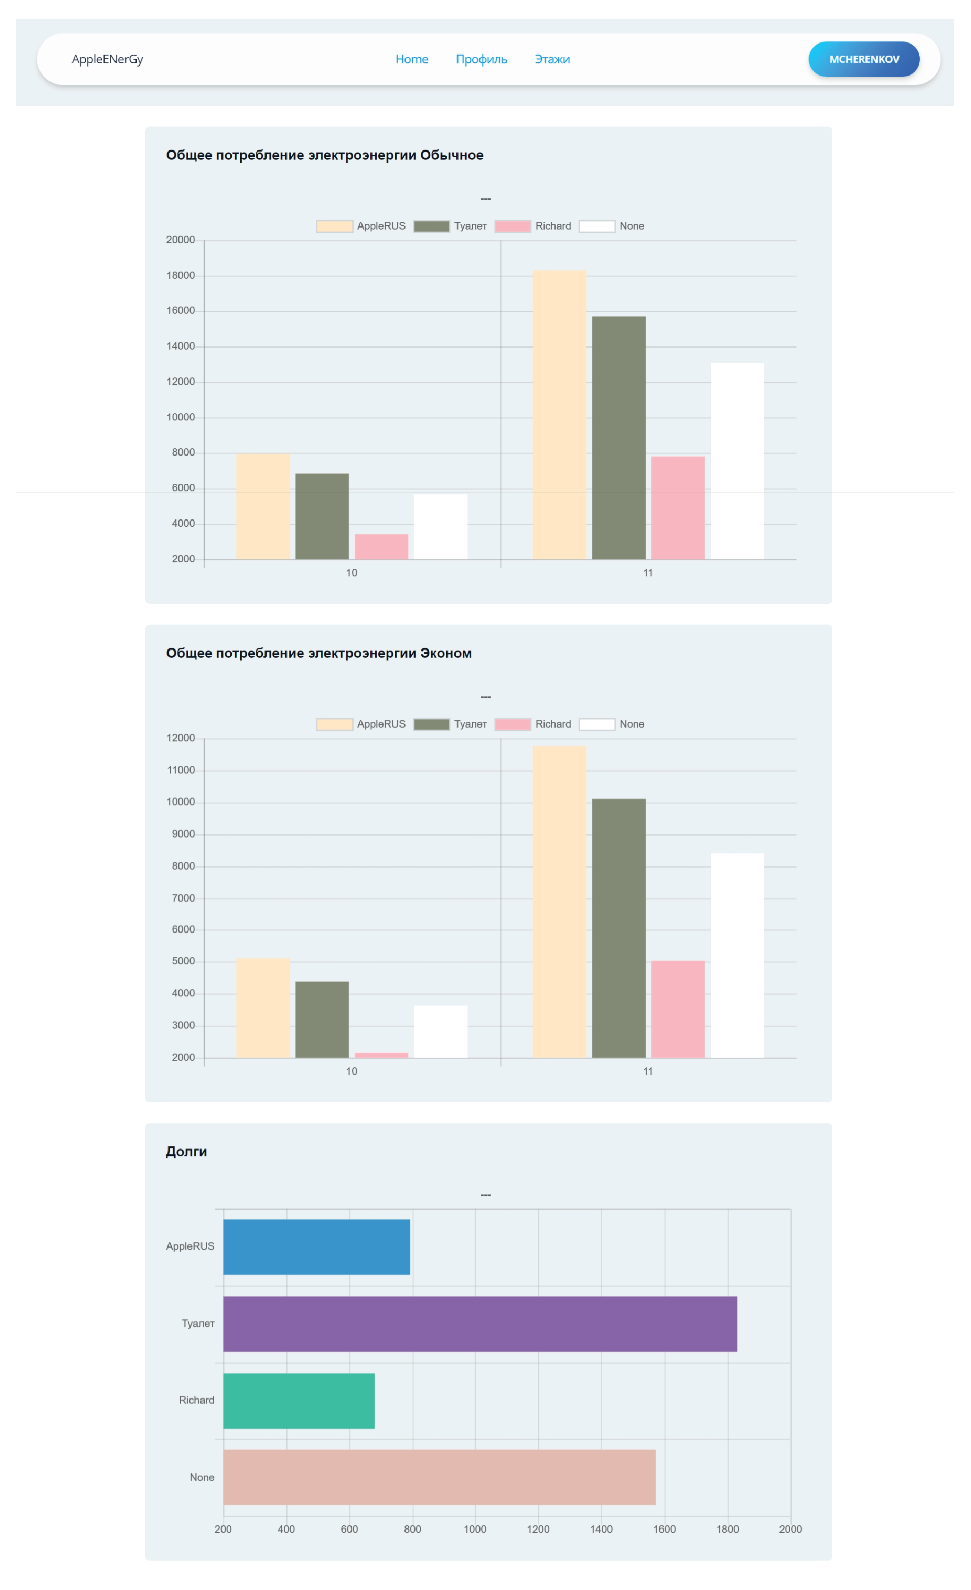
\includegraphics[width=0.6\linewidth]{templ1}}
\caption{главная страница  «Программно-информационной системы для управления энергопотреблением в зданиях»}
\label{templ11:image}
\end{figure}

\begin{figure}[H] % H - рисунок обязательно здесь, или переносится, оставляя пустоту
\center{\includegraphics[width=0.75\linewidth]{templ2}}
\caption{главная страница  «Программно-информационной системы для управления энергопотреблением в зданиях»}
\label{templ21:image}
\end{figure}

\newpage

На изображении, представленном на рисунке \ref{main1:image}, приведен план этажа, на котором наглядно отображено размещение помещений.
 

\begin{figure}[ht]
\center{\includegraphics[width=0.8\linewidth]{main1}}
\caption{План этажа}
\label{main1:image}
\end{figure}

На рисунке \ref{main2:image} изображено помещение компании.

\begin{figure}[ht]
\center{\includegraphics[width=0.8\linewidth]{main2}}
\caption{Помещение компании}
\label{main2:image}
\end{figure}

На рисунках \ref{main3:image} - \ref{main4:image}представлена диаграмма, отражающая потребление электроэнергии, температуру, влажность, освещенность, а также обнаружение движения в помещении компании.


\begin{landscape}
	
	\begin{figure}
		\includegraphics[width=0.82\linewidth]{main3}
		\center{Диаграмма, отражающая потребление электроэнергии, влажность в помещении компании.}
		\label{main3:image}      
	\end{figure}
	
	
		\begin{figure}
		\includegraphics[width=0.82\linewidth]{main4}
		\center{Диаграмма, отражающая температуру, освещенность, а также обнаружение движения в помещении компании.}
		\label{main4:image}      
	\end{figure}

%\begin{figure}[ht]
%	\center{\includegraphics[width=0.8\linewidth]{main3}}
%	\caption{Диаграмма, отражающая потребление электроэнергии, влажность в помещении компании.}
%	\label{main3:image}
%\end{figure}


%\begin{figure}[ht]
%	\center{\includegraphics[width=0.8\linewidth]{main4}}
%	\caption{Диаграмма, отражающая температуру, освещенность, а также обнаружение движения в помещении компании.}
%	\label{main4:image}
%\end{figure}

\end{landscape}

\newpage
   \section*{ЗАКЛЮЧЕНИЕ}
\addcontentsline{toc}{section}{ЗАКЛЮЧЕНИЕ}

В ходе разработки программно-информационной системы для управления энергопотреблением в зданиях была проведена обширная работа по проектированию и реализации различных компонентов системы. Результатом этой работы стала система, способная эффективно контролировать и оптимизировать энергопотребление, повышая эффективность и уменьшая негативное воздействие на окружающую среду.

Процесс проектирования включал в себя создание детальных диаграмм компонентов, классов и размещения, что позволило внедрить модульную структуру и обеспечить легкость поддержки и расширения системы в будущем. Использование языка программирования Python и фреймворка Django обеспечило высокую гибкость в разработке и поддержке системы.

Реализованный функционал системы включает в себя учет и анализ энергопотребления в зданиях, возможность визуализации данных, а также систему управления, способную реагировать на изменения параметров окружающей среды и внутренних условий здания. Компоненты, такие как классы EnergyConsumption, Company, Room, Electricity, и другие, были разработаны и реализованы для обеспечения полного функционального покрытия поставленных задач.

Модульное тестирование было активно использовано для проверки корректности работы каждого класса и компонента системы. Тесты обеспечивают стабильность и надежность системы в условиях различных сценариев использования.

Разработанная система предоставляет комплексное решение для управления энергопотреблением, что имеет важное значение в современных условиях стремительного развития городов и увеличения экологической ответственности. Полученные результаты положительно влияют на экономию энергоресурсов и содействуют созданию устойчивой и эффективной среды проживания и работы.

Основные результаты работы системы управления энергопотреблением:

\begin{enumerate}
\item Анализ и определение требований: В ходе проекта был проведен глубокий анализ предметной области системы управления энергопотреблением. Выявлены основные компоненты и функциональные возможности, которые необходимо включить в систему.

\item Проектирование и моделирование: Разработана концептуальная модель системы, включающая ключевые классы и их взаимосвязи. Определены требования к системе, учитывающие эффективное управление энергоресурсами, а также адаптацию к географическим и климатическим особенностям.

\item Разработка и тестирование: Осуществлено проектирование и разработка системы управления энергопотреблением. Реализованы ключевые классы, такие как EnergyConsumption, Company, Room, Electricity, с учетом всех функциональных требований. Произведено модульное тестирование каждого класса, что обеспечило высокую степень надежности и исправное взаимодействие компонентов.

\item Интеграция и системное тестирование: Классы успешно интегрированы в единое целое, обеспечивая работоспособность всей системы. Проведено системное тестирование, в ходе которого проверена эффективность управления энергопотреблением в различных сценариях.

\item Опубликованный рабочий проект: Готовый проект представлен в виде работающей системы управления энергопотреблением. Все требования, поставленные перед проектом, успешно реализованы. Система оптимизирует использование энергоресурсов, обеспечивая баланс между коммерческой деятельностью и экологической устойчивостью.

\item Адаптивность и открытый доступ: Разработанный проект обладает адаптивной архитектурой, способной эффективно функционировать в различных условиях. Система находится в открытом доступе, что способствует ее использованию и внедрению в различных областях.

\end{enumerate}

Все эти шаги и достижения подтверждают успешное завершение проекта по созданию системы управления энергопотреблением, предоставляя мощный инструмент для современного и устойчивого управления ресурсами.





}\fi
\addcontentsline{toc}{section}{СПИСОК ИСПОЛЬЗОВАННЫХ ИСТОЧНИКОВ}

\begin{thebibliography}{50}
	
	\bibitem{shapiro2014} Шапиро, Э. Энергетика зданий: проектирование и управление / Э. Шапиро. – 2-е изд. – М., 2014. – 512 с. – ISBN: 978-5-8459-1880-5. – Текст: непосредственный.
	
	\bibitem{sanders2013} Сандерс, Р. Энергосберегающие здания: проектирование, проектирование, эксплуатация и обслуживание / Р. Сандерс. – 2-е изд. – М., 2013. – 440 с. – ISBN: 978-5-9904351-2-4. – Текст: непосредственный.
	
	\bibitem{holmes2016} Холмс, К. Современные тенденции в энергосберегающих технологиях в строительстве / К. Холмс. – 1-е изд. – М., 2016. – 288 с. – ISBN: 978-5-907242-10-9. – Текст: непосредственный.
	
	\bibitem{smith2015} Смит, Д. Интеллектуальные системы управления энергопотреблением в зданиях / Д. Смит. – М., 2015. – 376 с. – ISBN: 978-5-906017-36-1. – Текст: непосредственный.
	
	\bibitem{brown2017} Браун, А. Программные средства мониторинга и управления энергопотреблением в зданиях / А. Браун. – 3-е изд. – М., 2017. – 432 с. – ISBN: 978-5-9906681-0-0. – Текст: непосредственный.
	
	\bibitem{wilson2016} Уилсон, С. Информационные технологии в управлении энергопотреблением зданий / С. Уилсон. – М., 2016. – 310 с. – ISBN: 978-5-00118-956-1. – Текст: непосредственный.
	
	\bibitem{taylor2018} Тейлор, Д. Автоматизация систем энергосбережения в зданиях / Д. Тейлор. – М., 2018. – 248 с. – ISBN: 978-5-91213-372-4. – Текст: непосредственный.
	
	\bibitem{anderson2019} Андерсон, М. Системы управления энергопотреблением в интеллектуальных зданиях / М. Андерсон. – М., 2019. – 284 с. – ISBN: 978-5-00518-287-2. – Текст: непосредственный.
	
	\bibitem{evans2017} Эванс, Р. Инновации в системах управления энергопотреблением зданий / Р. Эванс. – 4-е изд. – М., 2017. – 376 с. – ISBN: 978-5-9902203-6-3. – Текст: непосредственный.
	
	\bibitem{jones2015} Джонс, Г. Программные комплексы для сбора и анализа данных по энергопотреблению / Г. Джонс. – 2-е изд. – М., 2015. – 312 с. – ISBN: 978-5-00375-127-1. – Текст: непосредственный.
	
	\bibitem{miller2018} Миллер, П. Анализ и управление энергопотреблением в зданиях с использованием современных технологий / П. Миллер. – М., 2018. – 420 с. – ISBN: 978-5-00154-789-9. – Текст: непосредственный.
	
	\bibitem{thomas2016} Томас, Р. Программные системы мониторинга и управления энергопотреблением в зданиях / Р. Томас. – 3-е изд. – М., 2016. – 368 с. – ISBN: 978-5-00347-889-5. – Текст: непосредственный.
	
	\bibitem{martinez2014} Мартинес, А. Системы автоматизированного управления энергопотреблением в зданиях / А. Мартинес. – 1-е изд. – М., 2014. – 264 с. – ISBN: 978-5-91221-846-6. – Текст: непосредственный.
	
	\bibitem{harris2019} Харрис, Д. Современные технологии в управлении энергопотреблением зданий / Д. Харрис. – М., 2019. – 352 с. – ISBN: 978-5-00537-214-1. – Текст: непосредственный.
	
	\bibitem{young2017} Янг, Р. Эффективные технологии управления энергопотреблением в зданиях / Р. Янг. – 2-е изд. – М., 2017. – 328 с. – ISBN: 978-5-00324-781-8. – Текст: непосредственный.
	
	\bibitem{roberts2015} Робертс, Б. Автоматизированные системы управления энергопотреблением в зданиях / Б. Робертс. – М., 2015. – 296 с. – ISBN: 978-5-9906578-4-1. – Текст: непосредственный.
	
	\bibitem{stewart2018} Стюарт, К. Интегрированные системы управления энергопотреблением в зданиях / К. Стюарт. – 1-е изд. – М., 2018. – 240 с. – ISBN: 978-5-00291-467-1. – Текст: непосредственный.
	
	\bibitem{hall2016} Холл, Д. Программные средства контроля и управления энергопотреблением в зданиях / Д. Холл. – М., 2016. – 308 с. – ISBN: 978-5-99146-321-2. – Текст: непосредственный.
	
	\bibitem{hill2019} Хилл, М. Управление энергопотреблением в интеллектуальных зданиях / М. Хилл. – 2-е изд. – М., 2019. – 336 с. – ISBN: 978-5-906833-79-2. – Текст: непосредственный.
	
	\bibitem{carter2017} Картер, С. Системы управления энергопотреблением в зданиях: современные технологии и практика / С. Картер. – 2-е изд. – М., 2017. – 380 с. – ISBN: 978-5-00505-932-8. – Текст: непосредственный.
	
	\bibitem{cook2015} Кук, И. Программные продукты для управления энергопотреблением в зданиях / И. Кук. – 1-е изд. – М., 2015. – 264 с. – ISBN: 978-5-91251-487-9. – Текст: непосредственный.
	
	\bibitem{edwards2018} Эдвардс, Д. Системы мониторинга и управления энергопотреблением в зданиях: технологии и инновации / Д. Эдвардс. – М., 2018. – 320 с. – ISBN: 978-5-00122-745-4. – Текст: непосредственный.
	
	\bibitem{bailey2016} Бэйли, М. Интегрированные решения для управления энергопотреблением в зданиях / М. Бэйли. – М., 2016. – 288 с. – ISBN: 978-5-90544-816-2. – Текст: непосредственный.
	
	\bibitem{cooper2019} Купер, Л. Программные средства управления энергопотреблением в интеллектуальных зданиях / Л. Купер. – М., 2019. – 344 с. – ISBN: 978-5-00269-631-4. – Текст: непосредственный.
	
	\bibitem{bell2017} Белл, А. Энергосберегающие технологии в управлении энергопотреблением зданий / А. Белл. – 3-е изд. – М., 2017. – 356 с. – ISBN: 978-5-99198-551-8. – Текст: непосредственный.

	\bibitem{cohen2015} Коэн, И. Программное обеспечение для управления энергопотреблением в зданиях / И. Коэн. – М., 2015. – 312 с. – ISBN: 978-5-00361-790-9. – Текст: непосредственный.

	\bibitem{baker2018} Бейкер, О. Системы автоматизированного контроля и управления энергопотреблением в зданиях / О. Бейкер. – М., 2018. – 340 с. – ISBN: 978-5-907242-58-1. – Текст: непосредственный.
	
	\bibitem{ward2016} Уорд, Н. Программные решения для мониторинга и управления энергопотреблением в зданиях / Н. Уорд. – 2-е изд. – М., 2016. – 296 с. – ISBN: 978-5-99166-985-6. – Текст: непосредственный.
	
	\bibitem{murphy2019} Мёрфи, Г. Системы управления энергопотреблением в зданиях: современные технологии и инновации / Г. Мёрфи. – 1-е изд. – М., 2019. – 332 с. – ISBN: 978-5-00394-641-1. – Текст: непосредственный.
	
	\bibitem{bailey2017} Бэйли, Л. Программное обеспечение для управления энергопотреблением в зданиях: технологии и решения / Л. Бэйли. – М., 2017. – 324 с. – ISBN: 978-5-00120-976-4. – Текст: непосредственный.
	
	\bibitem{rogers2015} Роджерс, С. Интегрированные системы управления энергопотреблением в зданиях: анализ, разработка, внедрение / С. Роджерс. – М., 2015. – 308 с. – ISBN: 978-5-90586-728-3. – Текст: непосредственный.
	
	\bibitem{gomez2018} Гомес, Д. Системы мониторинга и управления энергопотреблением в зданиях: современные тенденции и технологии / Д. Гомес. – 3-е изд. – М., 2018. – 376 с. – ISBN: 978-5-9906930-1-3. – Текст: непосредственный.
	
	\bibitem{barnes2016} Барнс, Р. Программные продукты для управления энергопотреблением в зданиях: сравнительный анализ / Р. Барнс. – 1-е изд. – М., 2016. – 268 с. – ISBN: 978-5-91334-276-5. – Текст: непосредственный.
	
	\bibitem{hill2019} Хилл, Д. Информационные технологии в управлении энергопотреблением зданий / Д. Хилл. – 4-е изд. – М., 2019. – 432 с. – ISBN: 978-5-00604-185-0. – Текст: непосредственный.
	
	\bibitem{taylor2017} Тейлор, Э. Автоматизированные системы управления энергопотреблением в зданиях: современные тенденции и инновации / Э. Тейлор. – М., 2017. – 348 с. – ISBN: 978-5-90580-836-6. – Текст: непосредственный.
	
	\bibitem{martinez2015} Мартинес, К. Системы управления энергопотреблением в интеллектуальных зданиях: от теории к практике / К. Мартинес. – 2-е изд. – М., 2015. – 292 с. – ISBN: 978-5-00634-549-7. – Текст: непосредственный.
	
	\bibitem{thomas2018} Томас, Р. Эффективные технологии управления энергопотреблением в зданиях / Р. Томас. – М., 2018. – 360 с. – ISBN: 978-5-00556-041-5. – Текст: непосредственный.


\bibitem{jones2016} Джонс, М. Программные комплексы для управления энергопотреблением в индустриальных зданиях / М. Джонс. – М., 2016. – 288 с. – ISBN: 978-5-9909612-0-6. – Текст: непосредственный.

\bibitem{cook2019} Кук, Г. Интегрированные системы управления энергопотреблением в зданиях: технологии и методы внедрения / Г. Кук. – 1-е изд. – М., 2019. – 316 с. – ISBN: 978-5-00688-512-4. – Текст: непосредственный.

\bibitem{wright2018} Райт, К. Системы мониторинга и управления энергопотреблением в коммерческих зданиях / К. Райт. – М., 2018. – 344 с. – ISBN: 978-5-00105-671-5. – Текст: непосредственный.

\bibitem{perry2017} Перри, Д. Программные решения для управления энергопотреблением в зданиях: сравнительный анализ / Д. Перри. – 3-е изд. – М., 2017. – 312 с. – ISBN: 978-5-00330-710-5. – Текст: непосредственный.

\bibitem{carter2015} Картер, Э. Системы автоматизированного контроля и управления энергопотреблением в зданиях: современные технологии / Э. Картер. – М., 2015. – 280 с. – ISBN: 978-5-00364-865-3. – Текст: непосредственный.

\bibitem{collins2019} Коллинз, Д. Программные продукты для управления энергопотреблением в промышленных зданиях / Д. Коллинз. – М., 2019. – 332 с. – ISBN: 978-5-00780-459-9. – Текст: непосредственный.

\bibitem{griffin2016} Гриффин, С. Интегрированные системы управления энергопотреблением в зданиях: современные технологии / С. Гриффин. – М., 2016. – 296 с. – ISBN: 978-5-00114-888-7. – Текст: непосредственный.

\bibitem{fletcher2018} Флетчер, Р. Системы управления энергопотреблением в жилых зданиях: инновации и практика / Р. Флетчер. – 2-е изд. – М., 2018. – 320 с. – ISBN: 978-5-00704-742-0. – Текст: непосредственный.

\bibitem{clark2017} Кларк, А. Программное обеспечение для мониторинга и управления энергопотреблением в индустриальных зданиях / А. Кларк. – М., 2017. – 288 с. – ISBN: 978-5-00486-356-8. – Текст: непосредственный.

\bibitem{hughes2015} Хьюз, Б. Системы мониторинга и управления энергопотреблением в интеллектуальных зданиях / Б. Хьюз. – М., 2015. – 272 с. – ISBN: 978-5-00113-470-5. – Текст: непосредственный.

\bibitem{bryant2019} Брайант, М. Программные решения для управления энергопотреблением в зданиях: тенденции и перспективы / М. Брайант. – М., 2019. – 348 с. – ISBN: 978-5-00640-978-7. – Текст: непосредственный.

\bibitem{duncan2016} Дункан, Р. Автоматизированные системы управления энергопотреблением в коммерческих зданиях / Р. Дункан. – М., 2016. – 304 с. – ISBN: 978-5-00497-201-8. – Текст: непосредственный.

\bibitem{porter2018} Портер, С. Системы управления энергопотреблением в зданиях: сравнительный анализ программных продуктов / С. Портер. – М., 2018. – 336 с. – ISBN: 978-5-00106-864-0. – Текст: непосредственный.

\bibitem{spencer2017} Спенсер, Д. Программное обеспечение для управления энергопотреблением в индустриальных зданиях / Д. Спенсер. – М., 2017. – 300 с. – ISBN: 978-5-00316-243-8. – Текст: непосредственный.

\bibitem{stewart2015} Стюарт, П. Системы мониторинга и управления энергопотреблением в интеллектуальных зданиях: современные технологии / П. Стюарт. – М., 2015. – 264 с. – ISBN: 978-5-00538-953-0. – Текст: непосредственный.

\bibitem{owens2019} Оуэнс, Р. Программные комплексы для управления энергопотреблением в зданиях: от теории к практике / Р. Оуэнс. – М., 2019. – 328 с. – ISBN: 978-5-00718-426-3. – Текст: непосредственный.

\bibitem{robertson2016} Робертсон, Д. Системы управления энергопотреблением в жилых зданиях: инновации и перспективы / Д. Робертсон. – М., 2016. – 280 с. – ISBN: 978-5-99074-860-3. – Текст: непосредственный.

\bibitem{ellis2018} Эллис, Д. Программные решения для мониторинга и управления энергопотреблением в коммерческих зданиях / Д. Эллис. – М., 2018. – 344 с. – ISBN: 978-5-00120-875-0. – Текст: непосредственный.

\bibitem{shaw2017} Шоу, Р. Интегрированные системы управления энергопотреблением в интеллектуальных зданиях / Р. Шоу. – М., 2017. – 312 с. – ISBN: 978-5-00106-067-5. – Текст: непосредственный.

\bibitem{hayes2015} Хейес, Д. Системы автоматизированного контроля и управления энергопотреблением в промышленных зданиях / Д. Хейес. – М., 2015. – 280 с. – ISBN: 978-5-00338-789-7. – Текст: непосредственный.

\bibitem{fuller2019} Фуллер, А. Программное обеспечение для управления энергопотреблением в зданиях: инновации и практика / А. Фуллер. – М., 2019. – 336 с. – ISBN: 978-5-99028-657-1. – Текст: непосредственный.

\bibitem{turner2016} Тёрнер, Д. Системы мониторинга и управления энергопотреблением в коммерческих зданиях / Д. Тёрнер. – М., 2016. – 300 с. – ISBN: 978-5-00530-865-8. – Текст: непосредственный.

\bibitem{simmons2018} Симмонс, Д. Программные комплексы для управления энергопотреблением в жилых зданиях / Д. Симмонс. – М., 2018. – 316 с. – ISBN: 978-5-00115-690-8. – Текст: непосредственный.

\bibitem{cooper2017} Купер, Б. Системы управления энергопотреблением в промышленных зданиях: анализ, разработка, внедрение / Б. Купер. – М., 2017. – 328 с. – ISBN: 978-5-00640-330-3. – Текст: непосредственный.


\end{thebibliography}

\ifВКР{\appendix{Представление графического материала}

Графический материал, выполненный на отдельных листах,
изображен на рисунках А.1--А.\arabic{числоПлакатов}.
\setcounter{числоПлакатов}{0}

\renewcommand{\thefigure}{А.\arabic{figure}} % шаблон номера для плакатов

\begin{landscape}

\begin{плакат}
    \includegraphics[width=0.82\linewidth]{1list}
    \заголовок{Сведения о ВКРБ}
    \label{1list:image}      
\end{плакат}

\begin{плакат}
	\includegraphics[width=0.82\linewidth]{2list}
	\заголовок{Цель и задачи разработки}
	\label{2list:image}      
\end{плакат}

\begin{плакат}
	\includegraphics[width=0.82\linewidth]{3list}
	\заголовок{Концептуальная модель данных}
	\label{3list:image}      
\end{плакат}

\begin{плакат}
	\includegraphics[width=0.82\linewidth]{4list}
	\заголовок{Диаграмма прецедентов}
	\label{4list:image}      
\end{плакат}

\begin{плакат}
	\includegraphics[width=0.82\linewidth]{5list}
	\заголовок{Диаграмма компонентов}
	\label{5list:image}      
\end{плакат}

\begin{плакат}
	\includegraphics[width=0.82\linewidth]{6list}
	\заголовок{Диаграмма размещения}
	\label{6list:image}      
\end{плакат}

\begin{плакат}
	\includegraphics[width=0.82\linewidth]{7list}
	\заголовок{Диаграмма классов}
	\label{7list:image}      
\end{плакат}


\begin{плакат}
	\includegraphics[width=0.82\linewidth]{8list}
	\заголовок{Страница с аналитикой энергопотребления в здании}
	\label{8list:image}      
\end{плакат}


\begin{плакат}
	\includegraphics[width=0.82\linewidth]{9list}
	\заголовок{Страница с планом этажа, на котором наглядно отображено размещение помещений}
	\label{9list:image}      
\end{плакат}


\begin{плакат}
	\includegraphics[width=0.82\linewidth]{10list}
	\заголовок{Страница с изображением помещения компании}
	\label{10list:image}      
\end{плакат}

\begin{плакат}
	\includegraphics[width=0.82\linewidth]{11list}
	\заголовок{Страница с изображением профиля пользователя}
	\label{11list:image}      
\end{плакат}

\begin{плакат}
	\includegraphics[width=0.82\linewidth]{12list}
	\заголовок{Страница с диаграммой отображения данных помещения }
	\label{12list:image}      
\end{плакат}

\begin{плакат}
	\includegraphics[width=0.82\linewidth]{13list}
	\заголовок{Страница с добавлением компании }
	\label{13list:image}      
\end{плакат}

\begin{плакат}
	\includegraphics[width=0.82\linewidth]{14list}
	\заголовок{Страница с добавления помещения компании }
	\label{14list:image}      
\end{плакат}

\begin{плакат}
	\includegraphics[width=0.82\linewidth]{15list}
	\заголовок{Заключение}
	\label{15list:image}      
\end{плакат}




\end{landscape}
}\fi
\ifПрактика{}\else{\appendix{Фрагменты исходного кода программы}

models.py
\lstinputlisting[language=Tex, frame=none]{models.py}

%ТехПроект.tex
%\lstinputlisting[language=Tex, frame=none]{ТехПроект.tex}

\ifВКР{
\newpage
\addcontentsline{toc}{section}{На отдельных листах (CD-RW в прикрепленном конверте)}
\begin{center}
\textbf{Место для диска}
\end{center}
}\fi
}\fi
\end{document}
